\makeatletter
\newcommand{\lambdabar}{{\mathchoice
  {\smash@bar\textfont\displaystyle{0.25}{1.2}\lambda}
  {\smash@bar\textfont\textstyle{0.25}{1.2}\lambda}
  {\smash@bar\scriptfont\scriptstyle{0.25}{1.2}\lambda}
  {\smash@bar\scriptscriptfont\scriptscriptstyle{0.25}{1.2}\lambda}
}}
\newcommand{\smash@bar}[4]{%
  \smash{\rlap{\raisebox{-#3\fontdimen5#10}{$\m@th#2\mkern#4mu\mathchar'26$}}}%
}
\makeatother

\chapter{Optical Response of Gases of Stationary Atoms}

Except for some simplest configurations, it is impractical to analytically solve the problem of light propagation with re-scattering process in atomic gases. In this chapter, we will get to  the principle and practice of classical simulations of a number of different configurations and introduce some remarkable results.
 
\section{From quantum field theory to classical simulation}

Classical simulation is the main way to investigate cooperative atom response in a dense medium in our research. Under certain assumptions, for example, when photon recoil and saturation of the atoms are neglected, such an approach is valid both theoretically and practically.

In the limit of low intensity for driving light, the field-theory version of the Born-Markow approximation was introduced in an earlier paper~\cite{PhysRevA.55.513}, whereby one could find a hierarchy of equation of motion for an entire hierarchy of products of atomic operators. 

Starting from the full result of quantum field theory, by taking expectation values of the operator hierarchy, we obtain a hirerarchy of equations of motion for correlation functions. 

For a $J_g=0\rightarrow J_e=1$ atomic transition, we define the correlation functions as
\bea
\mathbf{P}_1(;\mathbf{r}_1)&=&\langle\psi^\dagger_g(\mathbf{r}_1)\mathbf{d}_{ge}\psi_e(\mathbf{r}_1)\rangle\equiv\langle\mathbf{P}^+(\mathbf{r}_1)\rangle,\nonumber\\
\mathbf{P}_2(\mathbf{r}_1;\mathbf{r}_2)&=&\langle\psi^\dagger_g(\mathbf{r}_1)\mathbf{P}^+(\mathbf{r}_2)\psi_g(\mathbf{r}_1)\rangle,\\
\mathbf{P}_3(\mathbf{r}_1,\mathbf{r}_2;\mathbf{r}_3)&=&\langle\psi^\dagger_g(\mathbf{r}_1)\psi^\dagger_g(\mathbf{r}_2)\mathbf{P}^+(\mathbf{r}_3)\psi_g(\mathbf{r}_2)\psi_g(\mathbf{r}_1)\rangle, \nonumber\\
&&\cdots,\nonumber
\eea
and also
\bea
\rho_1(\mathbf{r}_1)&=&\langle\psi^\dagger_g(\mathbf{r}_1)\psi_g(\mathbf{r}_1)\rangle,\nonumber\\
\rho_2(\mathbf{r}_1,\mathbf{r}_2)&=&\langle\psi^\dagger_g(\mathbf{r}_1)\psi^\dagger_g(\mathbf{r}_2)\psi_g(\mathbf{r}_2)\psi_g(\mathbf{r}_1)\rangle,\\
&&\cdots.\nonumber
\eea

$\mathbf{P}_k(\mathbf{r}_1,\cdots,\mathbf{r}_{k-1};\mathbf{r}_k)$ is the correlation function of the polarization at $\mathbf{r}_k$ and the atom density at $k-1$ positions $\mathbf{r}_1,\cdots,\mathbf{r}_{k-1}$, and $\rho_k$ is a $k$-point density correlation function. All of these are normally ordered. A hierarchy of equations for the correlation functions can be derived.

From the angle of classical physics, the correlations between the atoms are induced by scattered light, which in turn is essentially dipole radiation due to atomic polarization. In the limit of low light intensity, the response of the medium is isotropoic, and the equation of motion for the polarization reads
\bea
\dot{\mathbf{P}}(\mathbf{r}_1)=(i\Delta-\gamma)\mathbf{P}(\mathbf{r}_1)+i\zeta\rho(\mathbf{r}_1)\mathcal{E}_0(\mathbf{r}_1)+i\zeta\int d^3r_2\sf G(\mathbf{r}_1-\mathbf{r}_2)\mathbf{P}_2(\mathbf{r}_1;\mathbf{r}_2).
\label{CORE}
\eea

As before, $\Delta$ is the detuning from the atomic resonance, $\gamma$ is the HWHM linewidth of the transition, $\zeta=\mathcal{D}^2/\hbar$ and $\epsilon_0\mathcal{E}_0$ would be the electric displacement of the driving light if the matter were absent. $\sf G$ is the dipole field propagator, a $3\times 3$ matrix such that $\sf G(\mathbf{r}-\mathbf{r}^\prime)\mathbf{d}$ is the usual electric field at $\mathbf{r}$ from a dipole $\mathbf{d}$ at $\mathbf{r}^\prime$.

Eq.~\eq{CORE} is the first one of a succession of equations. In principle, the two-atom correlation $\mathbf{P}_2(\mathbf{r}_1;\mathbf{r}_2)$ is coupled to three-atom correlation functions, which are coupled to four-atom correlations, etc.

It's necessary to point out that the full quantum field theory even includes photon recoil on the center-of-mass motion of the atoms. In summary, in the case when photon recoil and saturation [population of the excited state(s)] are negligible, the level scheme of the atomic two-level transition is simple enough ($J_g=0\rightarrow J_e=1$), and the incoming light can be taken as classical (coherent state), classical electrodynamic applies for classical dipoles representing the atoms and for the electromagnetic fields. 

In the sections that follow, Eq.~\eq{CORE} will come up repeatedly as the foundation of all the classical simulations that we conducted, where we will formulate all the other factors in the simulations. 


\section{Preparation}
Keeping in mind the restrictions raised in the first section, in particular a sufficiently low intensity of the initially driving light, we therefore formulate our model entirely classically. In the present exposition we take all time dependent quantities as monochromatic, and write them in terms of complex amplitudes. For instance, the physical electric field at the position ${\bf r}$ would be expressed in terms of an amplitude vector ${\bf E}({\bf r})$ as
\beq
{\bf E}({\bf r},t) = \half {\bf E}({\bf r}) e^{-i\omega t} + {\rm c.\,c.}\,.
\eeq
The amplitude vectors may be complex, which allows for, say, circularly or elliptically polarized quantities as usual. 

With the given assumptions, according to the polarizability given by Eq.~\eq{POLARIZABILITY}, the dipole moment of an atom at point $\bf r$ is
\beq
{\bf d}_{{\bf r}} = -\frac{d^2}{\hbar(\Delta+ i\gamma)} {\bf E}({\bf r})\,,
\label{staticEtoD}
\eeq
where $d$ is the dipole moment matrix element for the transition. There is an explicit relation between the dipole matrix element, linewidth, and the wavenumber of resonant light $k_0 = \omega_0/c$. Now, the monochromatic light with the frequency $\omega$ need not be exactly on resonance, but dealing with near-resonant transitions in atoms we may usually ignore the difference between the wavenumber $k=\omega/c$ and the resonant wave number $k_0$. We therefore write the relation
\beq
\gamma = \frac{k^3 d^2}{6 \pi\hbar\epsilon_0}\,.
\eeq

The linewidth $\gamma$ describes damping of the dipole due to spontaneous emission. It has appeared more than once but here we have the explicit expression for the first time. $\gamma$ originates from quantum mechanics, but has a clear classical analog: An oscillating dipole radiates energy that should come from somewhere, namely from the energy of the oscillator. Even more to the present point, the linewidth may also be viewed as a result of radiation reaction, the field of the dipole falling back on the dipole and opposing its oscillations. This kind of an argument gives a quantitatively correct damping rate for a charged harmonic oscillator, albeit in a classical analysis one needs to drop manually an infinite in-phase field driving the dipole. Quantum mechanically, the infinite field is eliminated by renormalization.

Note that $\bf{E}(\bf{r})$ in Eq.~\eq{staticEtoD} denotes the electric field inside the sample. In traditional optics ~\cite{jackson,optics}, this field can be described by an effective electric field with local-field corrections based on the assumption of a continuous medium. Alternatively, if an atomic gas is treated as ensembles composed of point-like dipolar emitters, $\bf{E}(\bf{r})$ can also be interpreted as the total field at $\bf{r}$ including the incoming light plus the dipolar fields from all the other atoms~\cite{PhysRevLett.112.113603}. We will see intriguing comparisons between the two models later. 

%Moreover, Eq.~\eq{staticEtoD} is essentially a steady state solution to a more general equation of motion for the dipole moment.  New features brought by the atomic motions is the topic of the latter half of this paper.


Given the dipole moment induced on an atom, it will send out both an electric and a magnetic field that fall on the atom itself, causing radiation reaction, and on the other atoms as well. For instance, the electric field from a dipole at ${\bf r}_0$ is given by the familiar expression~\cite{jackson}
\bea
{\bf E}({\bf r; {\bf r}_0}) &=& \frac{1}{4\pi\epsilon_0}\left\{
k^2( \hat{\bf n}\times{\bf d}_{{\bf r}_0})\times \hat{\bf n}\,\frac{e^{ikR}}{R}\right.\nonumber\\
&&\left.+ [3\hat{\bf n}(\hat{\bf n}\cdot{\bf d}_{{\bf r}_0})-{\bf d}_{{\bf r}_0}]\left( \frac{1}{R^3}-\frac{ik}{R^2}\right)e^{ikR}
\right\};\\
R &=& |{\bf r}-{\bf r}_0|,\quad\hat {\bf n} = \frac{{\bf r}-{\bf r}_0}{R}\,.\label{DDIR}
\label{dipolarE}
\eea
In addition to the usual far-field radiation $\propto 1/R$ we will have to consider explicitly also the near fields $\propto 1/R^2$ and $\propto 1/R^3$.

In order to shorten the ensuing expressions, in our analysis we use the same units as also in the numerical calculations, setting
\beq
k = c = \hbar = \frac{1}{4\pi\epsilon_0} = 1\,.
\eeq
In particular, the unit of length derives from the free-space wavelength of the radiation $\lambda$ and equals $\lambda/2\pi$.
In these units the relation between the positive frequency parts of the electric and magnetic fields reads
\beq
{\bf B}({\bf r}) =-i\,\nabla\times{\bf E}({\bf r}) 
\eeq
the energy density and Poynting vector at the given field position read
\bea
\hbox{\sc e} &=& \frac{1}{16\pi}\, \Re[{\bf E}\cdot{\bf E}^*+{\bf B}\cdot{\bf B}^*],\\
{\bf S} &=& \frac{1}{8\pi}\, \Re[{\bf E}\times{\bf B}^*]\,,
\eea
and  the linewidth of the transition and dipole matrix element are related by
\beq
d = \sqrt{\frac{3\gamma}{2}}\,.
\eeq

The electric and magnetic fields of dipole radiation at position $\bf r$ are then given in dipole at ${\bf r}_0$ as
\beq
{\bf E}({\bf r}) = {\cal E}({\bf r},{\bf r}_0)\cdot {\bf d}_{{\bf r}_0},\quad
{\bf B}({\bf r}) = {\cal B}({\bf r},{\bf r}_0)\cdot {\bf d}_{{\bf r}_0}
\eeq
where $\cal E$ and $\cal B$ are $3\times3$ matrices with the elements
\bea
{\cal E}_{ij}({\bf r},{\bf r}_0) &=& \hat{\bf e}_i \cdot\left\{
(\hat{\bf n}\times \hat{\bf e}_j)\times\hat{\bf n} + [3\hat{\bf n}(\hat{\bf n}\cdot\hat{\bf e}_j)-\hat{\bf e}_j]\left( \frac{1}{R^2}-\frac{i}{R}\right)\right\}\frac{e^{iR}}{R}\,,\\
{\cal B}_{ij}({\bf r},{\bf r}) &=&\hat{\bf e}_i \cdot\hat{\bf n}\times\hat{\bf e}_j\left(1-\frac{1}{iR}\right)\,\frac{e^{iR}}{R}\,.
\eea
Here $R$ and $\hat{\bf n}$ are the distance from the source point to the field point and the unit vector pointing from the source point to the field point as before, Eq.~\eq{DDIR}, and $\hat{\bf e}_i$ are the cartesian unit vectors. One the other hand, given the electric field on an atom at ${\bf r}$, in the new convention of units the induced dipole moment reads
\beq
{\bf d}_{\bf r} = \alpha\,{\bf E}({\bf r}_0),\quad \alpha = -\frac{3}{2(\delta+i)}\,.
\label{STEADY}
\eeq
The sole material parameter that remains is the polarizability $\alpha$ expressed in terms of the detuning in units of the natural linewidth of the transition,
\beq
\delta = \Delta/\gamma\,.
\eeq
%\bea
%{\cal G}_{ij}({\bf r}) &=& \hat{\bf e}_i \cdot\left\{
%(\frac{\bf \br}{r}\,\times\! \hat{\bf e}_j)\!\times\!\frac{\bf \br}{r} + [3\frac{\bf \br}{r}(\frac{\bf \br}{r}\!\cdot\!\hat{\bf e}_j)\!-\!\hat{\bf e}_j]\left( \frac{1}{r^2}\!-\!\frac{i}{r}\right)\right\}\!\frac{e^{ir}}{r}\,,\\
%\eea
Consider now a collection of $N$ atoms at positions ${\bf r}_n$. The electric field on an atom at ${\bf r}_n$ equals the incoming field ${\bf E}_0$ plus the dipolar field from the other atoms, which is expressed in the set of equations
\beq
{\bf E}({\bf r}_n) = {\bf E}_0({\bf r}_n)+\sum_{m\ne n} {\cal E}({\bf r}_n,{\bf r}_m)\cdot{\bf d}({\bf r}_m)\,
\eeq
or
\beq
{\bf E}({\bf r}_n) = {\bf E}_0({\bf r}_n) + \alpha \sum_{m\ne n} {\cal E}({\bf r}_n,{\bf r}_m)\cdot{\bf E}({\bf r}_m)\,.\label{FEQ}
\eeq
The latter form makes a $3N\times3N$ set of linear equations for the cartesian components of the electric field at the positions of the atoms. Given the solutions ${\{\bf E}({\bf r}_n)\}_n$ we then have the electric and magnetic fields everywhere in space as
\bea
{\bf E}({\bf r})&=& \bE_0({\bf r}) + \alpha \sum_{n} {\cal E}({\bf r},{\bf r}_\alpha)\cdot{\bf E}({\bf r}_n),
\label{EF}\\
{\bf B}({\bf r}) &=& {\bf B}_0({\bf r}) + \alpha \sum_{n} {\cal B}({\bf r},{\bf r}_n)\cdot{\bf E}({\bf r}_n)\,,
\label{BF}
\eea
where ${\bf B}_0$ is the magnetic component of the incident field.

In brief, the plan of the present paper is to solve Eqs.~\eq{FEQ}, be it analytically or numerically, and analyze the resulting electromagnetic field, Eqs.~\eq{EF} and~\eq{BF}. 

\section{Calculation: Radiation from a single atom}
We begin with a single atom. It is driven by an incoming plane wave that propagates in the $x$ direction and is polarized in the $z$ direction, so that we have
\beq
{\bf E}_0({\bf r}) = E_0\, \hat{\bf e}_z\,  e^{i x},\quad {\bf r}_0 = 0\,.
\eeq
Since there are no other dipoles, the field driving the atom equals the external field
\beq
{\bf E}({\bf r}_0) = E_0\, \hat{\bf e}_z\,,
\eeq
and the dipolar fields are as usual. Denoting the unit vector from the origin to the point of observation and the position for the field observation as usual in terms of the spherical polar coordinates,
\bea
\hat{\bf r} &=& \sin\theta\cos\varphi\, \hat{\bf e}_x+ \sin\theta\sin\varphi\, \hat{\bf e}_y + \cos\theta\, \hat{\bf e}_z,\\
{\bf r} &=& r\,\hat{\bf r}\,,
\eea
the angular distribution of the outward flux of radiated energy at any given distance $r$ and the total radiated power are
\bea
F_1(\theta,\varphi) &=& r^2 \,\hat{\bf r}\cdot{\bf S} = \frac{9 |E_0|^2 \sin^2\theta}{32\pi(\delta^2+1)},\label{1DIPF}\\
P_1 &=& \int d\theta \sin\theta\,d\varphi\, F(\theta,\varphi) = \frac{3|E_0|^2}{4(\delta^2+1)}\label{1DIPP}\,.
\eea
These are uttterly familiar results, even if they might look unusual at first sight  because of our units.

Even if this is the case of a single atom and therefore presents no enhanced radiation due to neither interference nor cooperative effects, it is still instructive to see how the energetics works out, see also Ref.~\cite{CRA82}. Thus, the total electric and magnetic fields at point $\br$ are written as
\beq
\bE_T(\br) = \bE_D(\br) + \bE_0(\br),\, {\bf B}_T(\br) = \bf B_D(\br) + \bf B_0(\br),
\eeq
where the index $D$ denotes for the dipole radiation from the atom and index $0$ for the incoming field. The total Poynting vector therefore is
\beq
{\bf S}_T = \frac{1}{2\pi}\, \{\Re({\bf E_0}\times{\bf B_0}^*)+ \Re({\bf E_D}\times{\bf B_D}^*) + [\Re({\bf E_0}\times{\bf B_D}^*) +  \Re({\bf E_D}\times{\bf B_0}^*)]\}\,.
\eeq
The first term is due to the incoming field. When the corresponding energy flux is calculated over any surface (not containing any part of the source of the incoming field), the result is obviously zero. The second term is due to the radiation of the dipole alone, as if the incoming field were not present, and gives Eqs.~\eq{1DIPF}, \eq{1DIPP} for the flux and the total radiated power. The final term in square brackets gives the part of the Poynting vector that corresponds to the interference between the incoming and dipolar fields.

At large distances the interference term is the dominant contribution to the Poynting vector. It is quite complicated already for this  simple case and we will not write it down, but at a fixed large distance it may vary very rapidly with the angles and have a negative radial component, as if power were streaming toward the radiating dipole. There is  no guarantee that the Poynting vector is the local energy current as the continuity equation for energy only says that a suitable integral involving the Poynting vector over a closed surface equals the rate of change of the energy inside that surface. Nevertheless, one can  show analytically that the total power associated with the interference term equals $-P_1$. The total power coming  out of a closed (spherical, in our explicit calculations) surface surrounding the dipole equals $P_1-P_1=0$. This is as it should be, since evidently the dipole does not store or emit net energy but simply reradiates it.

\section{Calculation: Radiation from two atoms}
For two atoms an explicit solution for the radiation field exists no matter what are the incoming fields and the positions of the dipoles, but the general expression is complicated enough to be  completely useless. We discuss here as an example the special case in which a plane wave polarized in the $z$ direction and propagating in the $x$ direction strikes two atoms sitting on the $z$ axis. Specifically, we have the incoming field and the two positions for the dipoles
\beq
E_0({\bf r}) = E_0\, \hat{\bf e}_z\,  e^{i x},\quad {\bf r}_{\pm} = \pm\half\,\ell\,\hat{\bf e}_z\,.
\eeq

In this case the fields at the positions of the dipoles are
\beq
{\bf E}({\bf r}_\pm) = \frac{\ell ^3}{\ell ^3+2 i \alpha  \ell e^{i \ell }-2 \alpha  e^{i \ell }}\,E_0\,\hat{\bf e}_z\,.
\label{FOD}
\eeq
Since the dipolar field diverges with the decreasing distance from the source, one might expect that the field of one dipole on the other would diverge when the dipoles approach one another, but to opposite holds true: For a fixed detuning and hence fixed polarizability $\alpha$ the fields are actually proportional to $\ell^3$ as $\ell\rightarrow0$.

Fixed detuning, however, may not the most useful way of viewing the result. Instead, we insert the explicit expression of the polarization and write
\bea
{\bf E}({\bf r}_\pm) &=& \left\{
1 + \frac{3 e^{i\ell}(1-i\ell)/\ell^3}{\delta(\ell)-i\gamma(\ell)}
\right\}E_0\,\hat{\bf e}_z;\\
\Delta(\ell) &=& \Delta -3  \left[\frac{\cos (\ell )}{\ell ^3}+\frac{\sin (\ell )}{\ell
   ^2}\right] \gamma,\nonumber\\
\gamma(\ell) &=&\left[1+\frac{3 \sin (\ell )}{\ell ^3}-\frac{3 \cos (\ell )}{\ell ^2}\right]\gamma \,.
\label{GAMMAL}
\eea
This shows our first instance of collective shift and broadening of the resonance of the atoms as a result of the radiation from on dipole falling on the other. The sines and cosines clearly originate from retardation, propagation delay of light between the atoms. In the limit $\ell\rightarrow0$ we have the expansions, keeping the leading terms in real and imaginary parts,
\beq
\Delta(\ell)-\Delta \simeq -\frac{3\gamma}{\ell^3},\,\gamma(\ell) \simeq 2\gamma\,.
\eeq
The shift $\Delta(\ell)-\Delta$ diverges as  $\ell^{-3}$, which clearly reflects the dipole-dipole interactions between the atoms. On the other hand, the linewidth doubles.

Moving on to the energy flux of in the far field and the radiated power, we find after some tedious algebra (even with Mathematica) the expressions
\bea
F_2 &=& \frac{9 \gamma ^2 |E_0|^2 \cos ^2\!\left[\frac{1}{2} \ell  \cos
   (\theta )\right] \sin ^2(\theta )}{8 \pi  \left[\Delta (\ell )^2+\gamma (\ell )^2\right]},\\
P_2 &=&\frac{3 \gamma\,\gamma(\ell)|E_0|^2 }{2[\Delta^2(\ell)+\gamma^2(\ell)]}\,.
\eea
The angular distribution of the radiation, normalized in such a way that $\int_0^\pi d\theta\,\sin\theta P(\theta)=1$, reads
\beq
P(\theta;\ell) = \frac{3\gamma}{2\gamma(\ell)}\left[\frac{1}{2} \ell  \cos
   (\theta )\right] \sin ^2(\theta )\,.
\eeq
This shows the dipole radiation pattern modulated by the interference of the radiation from the two dipoles. See the demonstration in Fig.~\ref{DipoleRadiations}. For $\ell=0$ we have the usual dipole radiation pattern. With increasing $\ell$ the interference first concentrates the radiation more to the $\theta=\pi$ plane perpendicular to the dipole. With increasing $\ell$ the side lobes grow numerous, and the overall angular distribution pattern rounds out.

\begin{figure}[h!]
\begin{center}
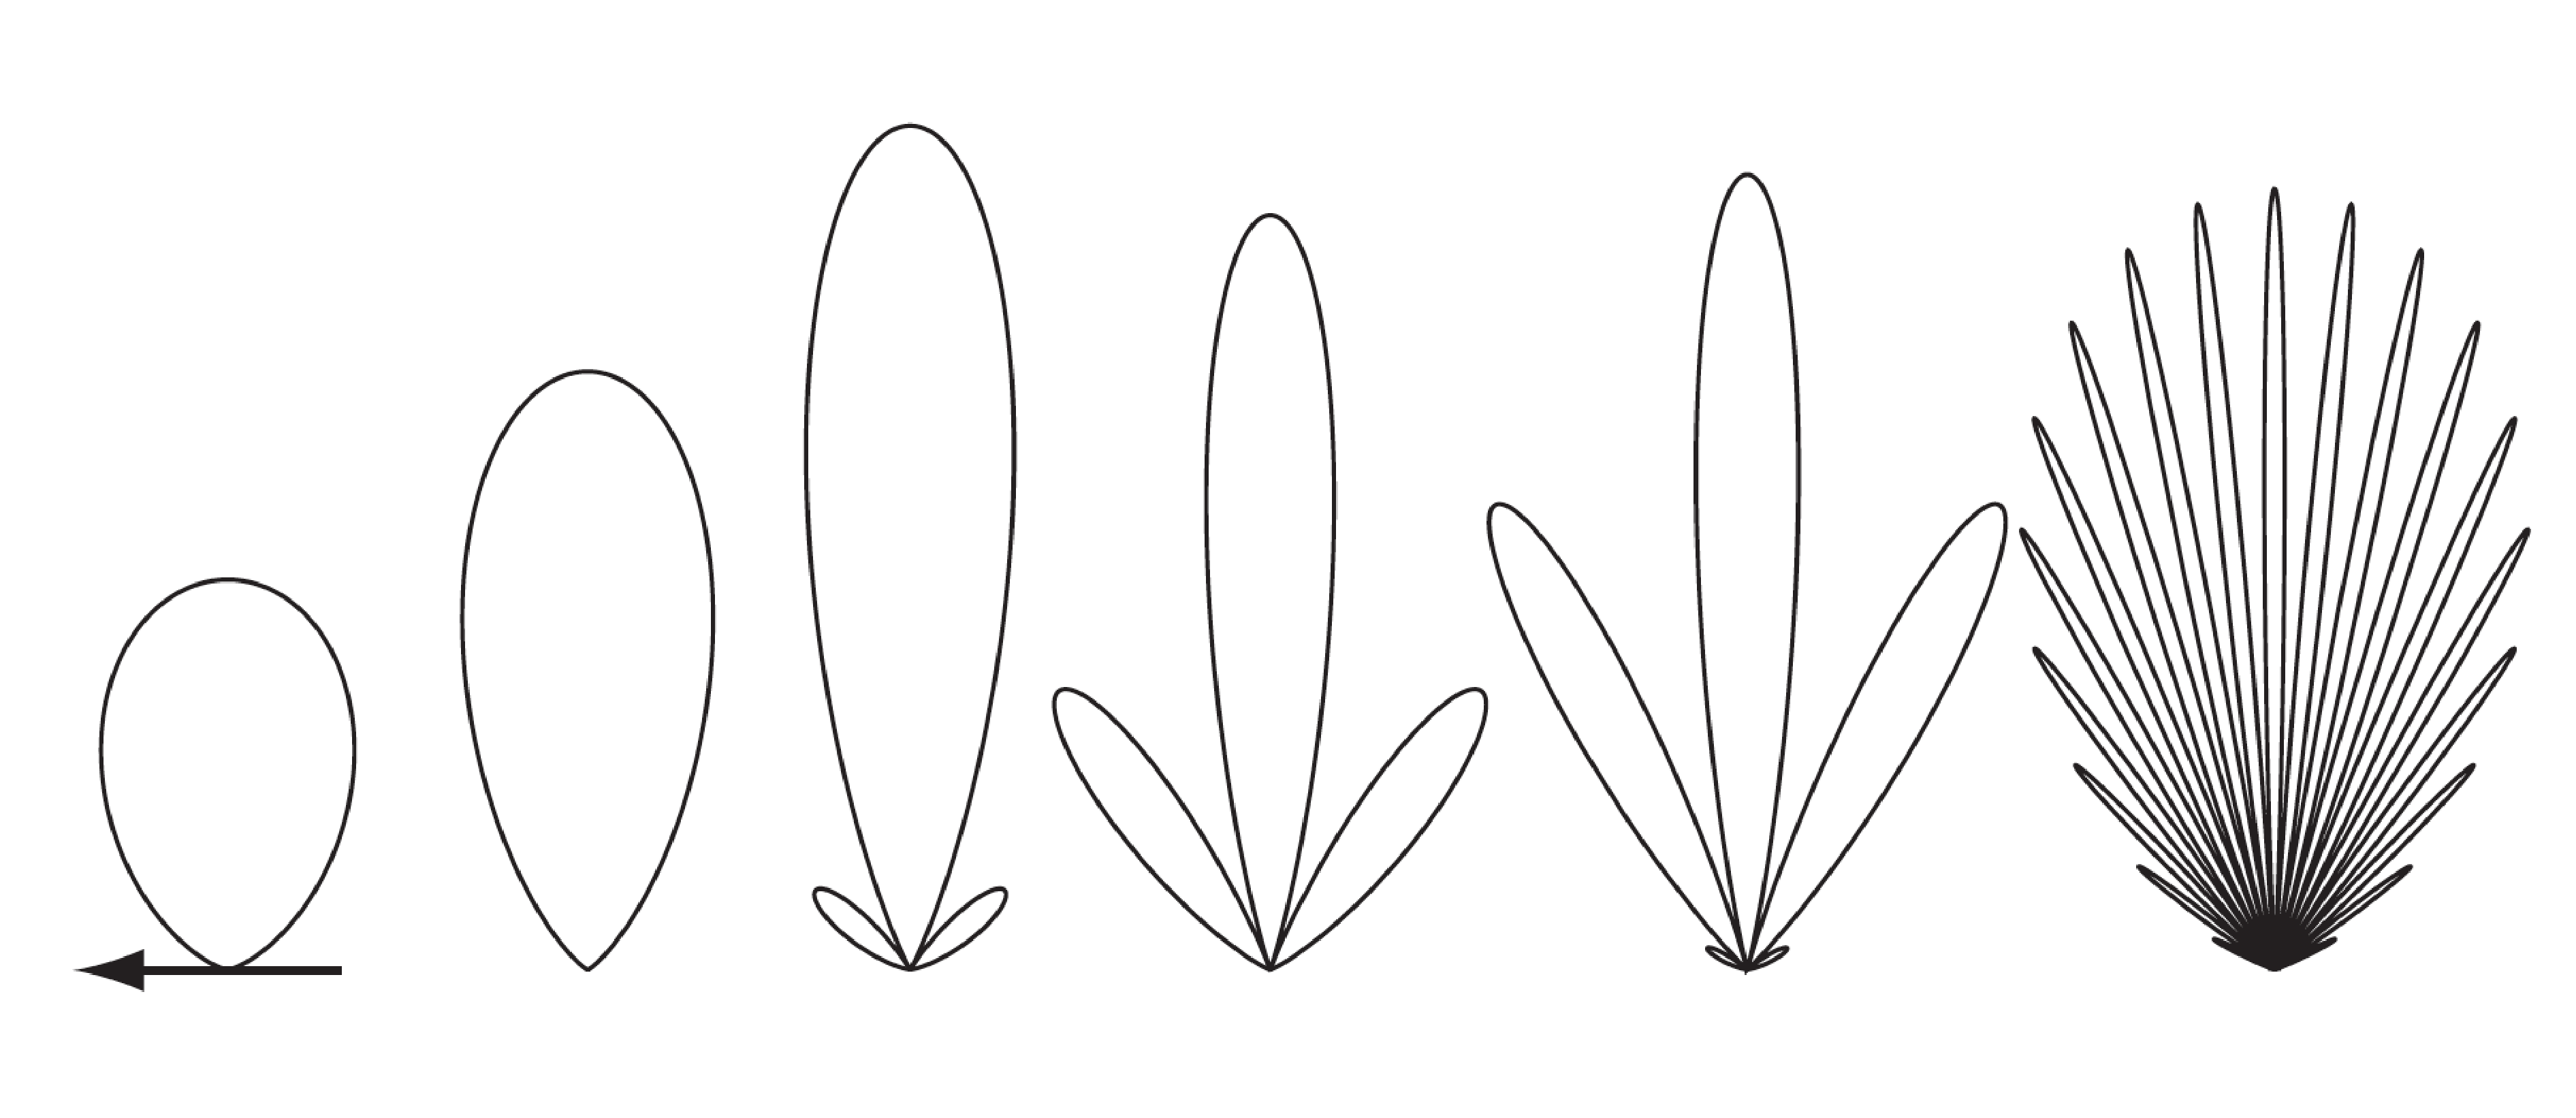
\includegraphics[width=0.8\textwidth]{two_atoms.pdf}
\end{center}
\caption[Radiation patterns for two dipoles]{Normalized radiation patterns $P(\theta;l)\sin\theta$ for the two dipoles for the distances between the dipoles $l=0,\pi,2\pi,3\pi,4\pi$, and $20\pi$ (left to right). These are a polar plots for $\theta\in[0,\pi]$,with the direction of the dipole and the $z$ axis denoted by the arrow in the $l=0$ graph.}
\label{TWOATOMS}
\end{figure}

As to the radiated power, the detuning from the single-atom resonance shifted by the co-operative effects is the true measure of resonance effects. We momentarily assume that this shift of reference point is implicit in the expressions of the energetics of the radiation, and simply replace $\Delta(\ell)\rightarrow\Delta$. On the other hand, if there were no co-operative effects or interference between the radiations of the two dipoles, the total radiated power would simply be twice the radiated power from one dipole under the same field. The ratio of these quantities
\beq
C = \frac{P_2}{2 P_1} = \frac{\gamma(\ell)[\Delta^2+\gamma^2]}{\gamma[\Delta^2+\gamma^2(\ell)]}
\eeq
is a reasonable measure of cooperativity, with $C=1$ applying to completely independent radiators.

The explicit expression follows immediately from Eq.~\eq{GAMMAL}. Since in the limit $\ell\rightarrow\infty$ we have $\gamma(\ell)\rightarrow\gamma$, we find $C\rightarrow1$ as expected. In the opposite limit $\ell\rightarrow0$ we have $\gamma(\ell)\rightarrow 2\gamma$, and the co-operativity depends in an essential manner on the detuning. If $|\Delta|\ll\gamma$, we have $C\simeq\half$. This means that on resonance the two atoms together radiate the same power as one single atom. On the other hand, with $|\Delta|\gg\gamma$, we have $C\simeq2$, and the two-atom sample radiates twice as much power as two independent atoms would. In fact, in this limit the radiated power can be expressed at all detunings as
\beq
P_2 = \frac{3 |E_0|^2}{2\{[\Delta/\gamma(\ell)]^2+1\}}\,,
\eeq
as if we had a single dipole with the dipole moment matrix element equal to $\sqrt2$ times the original dipole moment matrix element. Now, it is well known that on resonance the cross section for light scattering is independent of the dipole moment matrix element, so the cross section and scattered power are both independent of the dipole matrix element. On the other hand, far-off resonance the scattered power is in fact proportional to the square of the dipole matrix element times the linewidth, and as such is proportional to the fourth power of the matrix element. Hence, the power from two atoms is four times the power from one atom, or twice the power from two independent atoms. The $\ell\rightarrow0$ limit is fully compatible with the observation that the two atoms have merged into one and the dipole matrix element has been multiplied by $\sqrt2$, with the proviso   that, as a result of atom-atom interactions, there is a shift of the resonance that diverges in the limit $\ell\rightarrow0$.

There is an interesting little puzzle here as well: One would imagine that the when one simply joins the two atoms, the dipole moment matrix element should, perhaps, be twice the matrix element for a single atom, not multiplied by $\sqrt 2$. Granted, in quantum mechanics, when restricted to the state space of collective states that are invariant under the exchange of the two atoms, the factor in fact is $\sqrt2$. But here we have a completely {\em classical\/} situation. Does everything fit in?

For an answer, let us momentarily take a variation of the classical Lorentz mode for a dipole, namely two classical charged particles with charge $q$ moving in the $z$ direction. Both particles are bound to their equilibrium positions with assumedly immovable neutralizing charges so that there are restoring forces proportional to the square of the of natural frequency $\omega_0$ common to both of the oscillators. By a suitable choice of the origins of the coordinates, we make the equilibrium positions equal to zero. Nonetheless, we assume that in actuality the dipoles  sit back to back as in the example of the present section, and much closer than the wavelength of the driving light from one another. The fields from one dipole, the moving charge and the stationary "nucleus", then add up to a force that attempts to move the other charge in the same direction. We characterize this force by the frequency $\Omega$. Finally, we assume that both of the dipoles are driven by the same external field $E$ at the freqency $\omega$. The equations of motion for the positive-frequency components of the positions of the two charges are then
\bea
\ddot{z}_1 = -\omega_0^2 z_1+ \Omega^2 z_2 + \frac{qE}{2}e^{-i\omega t},\label{INDIVDIP1}\\
\ddot{z}_2 = -\omega_0^2 z_2+ \Omega^2 z_1 + \frac{qE}{2}e^{-i\omega t}\,.
\eea
In terms of the normal modes
\beq
\eta_\pm = \frac{1}{\sqrt 2} (z_1 \pm z_2)
\eeq
the equations of motion read
\bea
\ddot{\eta}_+ &=& -(\omega_0^2-\Omega^2)\eta_+ +\frac{qE}{\sqrt2} e^{-i\omega t},\label{COLLDIPP}\\
\ddot{\eta}_- &= &-(\omega_0^2+\Omega^2)\eta_-\,.
\eea
The resonance of the two modes $\eta_\pm$ are  shifted  in the opposite directions by the interaction between the dipoles. Besides, the ``nonradiating'' mode $\eta_-$ does not couple to the driving field at all. 

Let us now assume that there is some damping in the system that eventually leads to equilibrium, but which is otherwise negligible; for instance that we drive the dipoles off resonance. Then there is no excitation of the mode $\eta_-$. Moreover, a comparison of Eqs.~\eq{COLLDIPP} and~\eq{INDIVDIP1} with $\Omega=0$ shows that for the same driving field strength $E$ and for the same detuning of the frequency $\omega$ from the respective resonance frequencies $\sqrt{\omega_0^2-\Omega^2}$ and  $\omega_0$, the steady-state oscillation amplitude of the collective mode $\eta_+$ would be a factor of $\sqrt 2$ larger that the amplitude for a single dipole. This is ostensibly the $\sqrt 2$ for the collective response in quantum mechanics, but the normal modes are an auxiliary construct and as such have no a priori meaning in classical mechanics. We therefore consider the original displacement $z_1$ and $z_2$. These oscillate in phase and with the same amplitude as would one dipole, for the same detuning from resonance. The total radiated electric field from the two dipoles will thus be twice the field from one dipole and the radiated power is multiplied by four. Everything is as it should be.


\section{Radiation Power of Gaussian Clouds of Atoms}


\subsection{Continuous Medium}

For the more general problem of $N$-atom gases, let us start with a hypothetical model with continuous spatial distribution of atoms.

In terms of macroscopic electromagnetism, there is a monochromatic polarization of the sample
\beq
{\bf P}({\bf r},t) = \half\varrho({\bf r}) \,{\bf d}({\bf r})e^{-i\omega t} + {\rm c.c.}\,,
\eeq 
where $\varrho({\bf r})$ is the density of the sample  and $\bf d({\bf r})$ is the positive-frequency component of the eletcric dipole of an atom at the position $\bf r$. Taking the atoms  to reside around the origin of the coordinates, in the far field with $r\gg \lambda$ and $r\gg R$, the terms  $\propto 1/R^2$ and $\propto 1/R^3$ in Eq.~\eq{dipolarE} would vanish and the it gives the positive component of the field radiated by this polarization in the form
\bea
{\bf E}_R({\bf r})&\simeq&\frac{e^{ir}}{r} \int d^3r'\,e^{-i  \hat{\bf r}\cdot {\bf r}'}\varrho({\bf r}')
\, [\hat{\bf r}\times{\bf d}({\bf r}')]\times\hat{\bf r}\,;
\label{SCATFIELD}
\eea
$\hat{\bf r}={\bf r}/r$ is the unit vector that points from the source at $\simeq 0$ to the field point. 

For easy analysis, we model the density with a Gaussian,
\beq
\varrho({\bf r}) = \frac{3\sqrt3N}{2\sqrt2\pi^{3/2} R^3}\, e^{-\frac{3r^2}{2R^2}}\,,
\eeq
where $N$ is the atom number. In the limit $kR\gg1$ there will be a narrow cone of radiation around the direction of the incoming beam; let us denote the angle from the incident beam by $\theta$. The parametrization is chosen in such a way that the rms value of $|\br|$ equals $R$. 

For a tangible example, let us take a $\sigma_+$ circularly polarized plane wave propagating in the $z$ direction, writing
\beq
\bE_0(\br) = E_0\, e^{iz}\,\hat{\bf e}_+;\quad \hat{\bf e}_+=\frac{1}{\sqrt{2}}(\hat{\bf e}_x - i \hat{\bf e}_y)\,.
\label{incomingE}
\eeq
Accordingly, 
\bea
{\bf d}({\bf r})=\alpha\bE_0(\br)=\alpha E_0\, e^{iz}\,\hat{\bf e}_+;
\eea
Now we turn back to the radiated field:
\bea
{\bf E}_R({\bf r})&=&\frac{e^{ir}}{r}\int d^3r^{\prime} e^{-i\hat {{\bf n}} \cdot {\bf r}^{\prime}} \rho({\bf r^\prime}) [ \hat { \bf n} \times  {\bf d}({\bf r}^{\prime}) ]  \times \hat {\bf n}\nonumber\\
&=&\frac{3\sqrt{3}\alpha NE_0e^{ir}[ (\hat { \bf n} \times \hat{{\bf e}}_+)  \times \hat {\bf n}]}{2\sqrt{2}\pi ^{3/2}R^3r}\int d^3r^{\prime} e^{-i\hat {{\bf n}} \cdot {\bf r}^{\prime}}e^{iz}e^{\frac{-3r^{\prime2}}{2R^2}}\nonumber\\
&=&\frac{\alpha NE_0e^{ir-\frac{1}{3}R^2(1-\cos \theta)}}{r}[ (\hat { \bf n} \times \hat{{\bf e}}_+)  \times \hat {\bf n}].
\eea
The magnitude of the Poynting vector is 
\bea
S_C({\bf r})&=&\frac{|{\bf E}_R|^2}{8\pi}=\frac{\left|\alpha\right|^2N^2 E_0^2 e^{-\frac{2}{3}R^2(1-\cos \theta)}|(\hat { \bf n} \times \hat{\bf e}) \times \hat {\bf n} |^2}{8 \pi r^2} \nonumber\\
&=&\frac{\left|\alpha\right|^2N^2 E_0^2 e^{-\frac{2}{3}R^2(1-\cos \theta)} (1+\cos^2 \theta)}{16 \pi r^2};  
\eea
The total power of the radiation is readily obtained by
\bea
P_C&=&\int r^2 S_C({\bf r}) d^2\Omega\nonumber\\
&=&\frac{3\left|\alpha\right|^2N^2E_0^2\left[(4R^4-6R^2+9)-e^{-\frac{4R^2}{3}}(4R^4+6R^2+9)\right]}{32R^6}.
\eea
Here, the intensity of the observation light scales with the square of the atom number, $N^2$. This is similar to the important characteristic of superradiance. However, it's early for a conclusion now. Let us check a more realistic problem, where we have discrete atoms instead of a over simplified continuous medium.

\subsection{Independent Radiators}
Suppose we have collection of $N$ identical dipoles sitting at the positions ${\bf r}_i$ in the incoming field, and that each of these dipoles radiate a field ${\bf E}_i({\bf r})$ {\em independently\/} of one another, i.e., with no co-operative effects. The total dipolar field at the point ${\bf r}$ is then simply
\beq
{\bf E}_D({\bf r}) = \sum_i {\bf E}_i({\bf r})\,.
\eeq
Suppose we are in the far field when the Poisson vector is obviously radial and its absolute value is related in the same simple way to the square of the electric field as for a single dipole. The Poynting vector for the dipolar field then points radially outwards, and has the absolute value
\bea
S_D(\br) &=& \frac{1}{8\pi} \bE_D(\br)\cdot\bE_D^*(\br )\nonumber\\
&=& \frac{1}{8\pi} \sum_{i,j} \bE_i(\br)\cdot\bE_j ^*(\br)
\eea
It may be that the atoms, in fact, reside in some fixed configuration, but for a gaseous sample it is more physical to take them to have some random position distribution in space. We take the position of each atom to be a random variable independent of the positions of the other atoms, governed by same probability density function $f(\br)$. Then the average outward energy flux (over many samples of the gas) is given by
\bea
8 \pi\bar{S}_D &=&\left\langle
 \sum_{i\ne j} \bE_i(\br)\cdot\bE_j^*(\br)+\sum_i \bE_i(\br)\cdot\bE_i^*(\br)
\right\rangle\nonumber\\
&=&
 \sum_{i\ne j} \left\langle\bE_i(\br)\right\rangle
\cdot\left\langle\bE_j^*(\br)\right\rangle +
\sum_{i} \left\langle\bE_i(\br)\cdot\bE^*_i(\br)\right\rangle\nonumber\\
&=&N(N-1)|\left\langle \bE_i(\br)\right\rangle|^2 + N \left\langle\bE_i(\br)\cdot\bE^*_i(\br)\right\rangle\,.
\eea
The first term represents coherent scattering, as if the atom was spread out to a continuous dielectric material with the spatial shape specified by $f(\br)$. It arises from adding the fields of different radiators, and is essentially proportional to $N^2$. The second term $\propto N$ is for incoherent scattering, basically the sum of intensities radiated by the individual atom. It is present because the gas is not a continuous dielectric medium, but consists of discrete scatterers.

Incidentally, while this argument may not be as widely known as it deserves to be, it is far from new: Einstein used it to demonstrate the atomic (molecular) nature of matter when it was still under doubt. The blue sky comes from incoherent scattering. If air were a continuous dielectric medium, it would not scatter sunlight sideways, and the sky would be black.

For comparison purposes, we apply the same incoming light as in Eq.~\eq{incomingE} and the position distribution for the atoms is still taken to be Gaussian,
\beq
f(\br) = \frac{3\sqrt3}{2\sqrt2\,\pi^{3/2}R^3}\,e^{-\scriptstyle\frac{3r^2}{2R^2}}\,.
\eeq
Given the usual polarizability $\alpha$, the far field (the $1/r$ part of dipole radiation) averaged over the position of the atom, the absolute square of the former, and the  absolute square  of the field averaged over the positions give
\bea
\langle \bE_i(\br)\rangle &=& \alpha E_0 e^{ir-\hbox{$\frac{1}{3}$}R^2(1-\cos\theta)}[(\hat{\bf r}\times\hat{\bf e}_+)\times\hat{\bf r}]\,\frac{e^{ir}}{r},\\
|\langle \bE_i(\br)\rangle|^2 &=& \frac{|\alpha |^2| E_0|^2[3+\cos (2 \theta )] e^{\frac{2}{3} R^2 [\cos (\theta
   )-1]}}{4 r^2},\\
   \langle |\bE_i(\br)|^2\rangle &=& \frac{|\alpha |^2| E_0|^2[3+\cos (2 \theta )]}{4 r^2}\,.
\eea
The total radiated power then becomes
\bea
P_N&=&\frac{|\alpha|^2 |E_0|^2}{3}\Bigg\{
N(N-1)\frac{9\left[(4R^4-6R^2+9)-e^{-\frac{4R^2}{3}}(4R^4+6R^2+9)\right]}{32R^6}\nonumber\\
&&+N\Bigg\}\,.
\label{PN}
\eea

\begin{figure}[h!]
\begin{center}
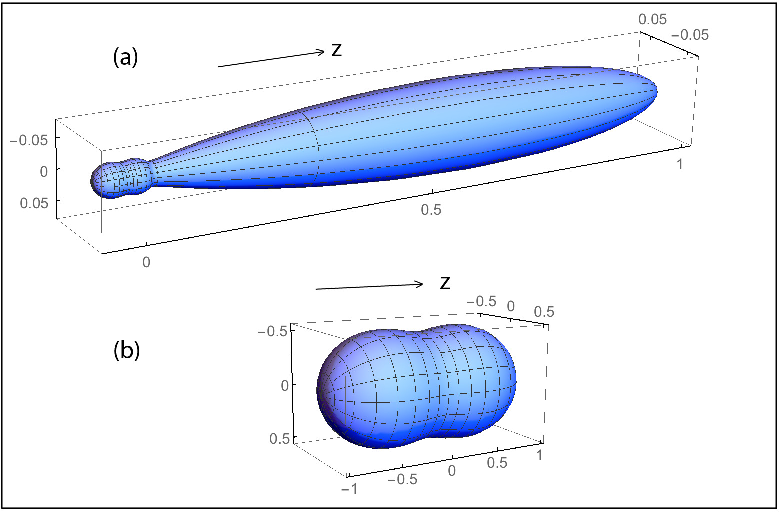
\includegraphics[width=\textwidth]{angular.pdf}
\end{center}
%\caption{Log-log plot of the total radiated power vs. the number of atoms from two types of models. $R$=1 and $\delta=600$ in both cases. The solid line is the result of Eq.~\eq{PN}. Ret dots denote the results from simulations.}
\caption{Normalized radiation patterns $P_N(\theta,R)\sin\theta$ for two Gaussian samples with $kR=10$ in (a) and $kR=0.1$ in (b). For both cases, the number of atoms $N=20$ and $\delta=600$.}
\label{ANGULAR}
\end{figure}


The main utility of these formulae is that they will serve as references to which to compare the numerical results. A few incidental results could be noted, however. As shown in Fig.~\eq{ANGULAR}, first, the intensity of the radiation in the forward direction, $\theta=0$, coherent and incoherent component, add up to exactly $N^2$ times the intensity from a single atom. The bigger the sample, the narrower the cone in the direction $\theta=0$ for coherent scattering. The sample acts as an antenna that directs the radiation in the forward direction. However, the total power decreases with increasing size of the cloud. Conversely, in the limit $R\rightarrow0$ the intensity in all directions is enhanced by a factor $N^2$, and of course so is the total power. People familiar with the Dicke cooperative regime might erroneously interpret such an enhancement as a cooperative phenomenon, which it is not since in this example we have simply added the fields from independent radiators.

%Last but not least, the difference between the continuous medium model and the independent radiators model in the total scattering power is given by
%\bea
%P_N-P_C&=&\frac{N\left|\alpha\right|^2E_0^2}{3}\nonumber\\
%&&\cdot\left\{1-\frac{9\left[(4R^4-6R^2+9)-e^{-\frac{4R^2}{3}}(4R^4+6R^2+9)\right]}{32R^6}\right\}
%\label{diffNandC}
%\eea

\subsection{Simulation of the scattered light power} 

When the dipolar fields from all the other radiators are taken into account, an analytical calculation for the total power is impractical and we have to turn to simulations. 

\begin{figure}[h!]
\begin{center}
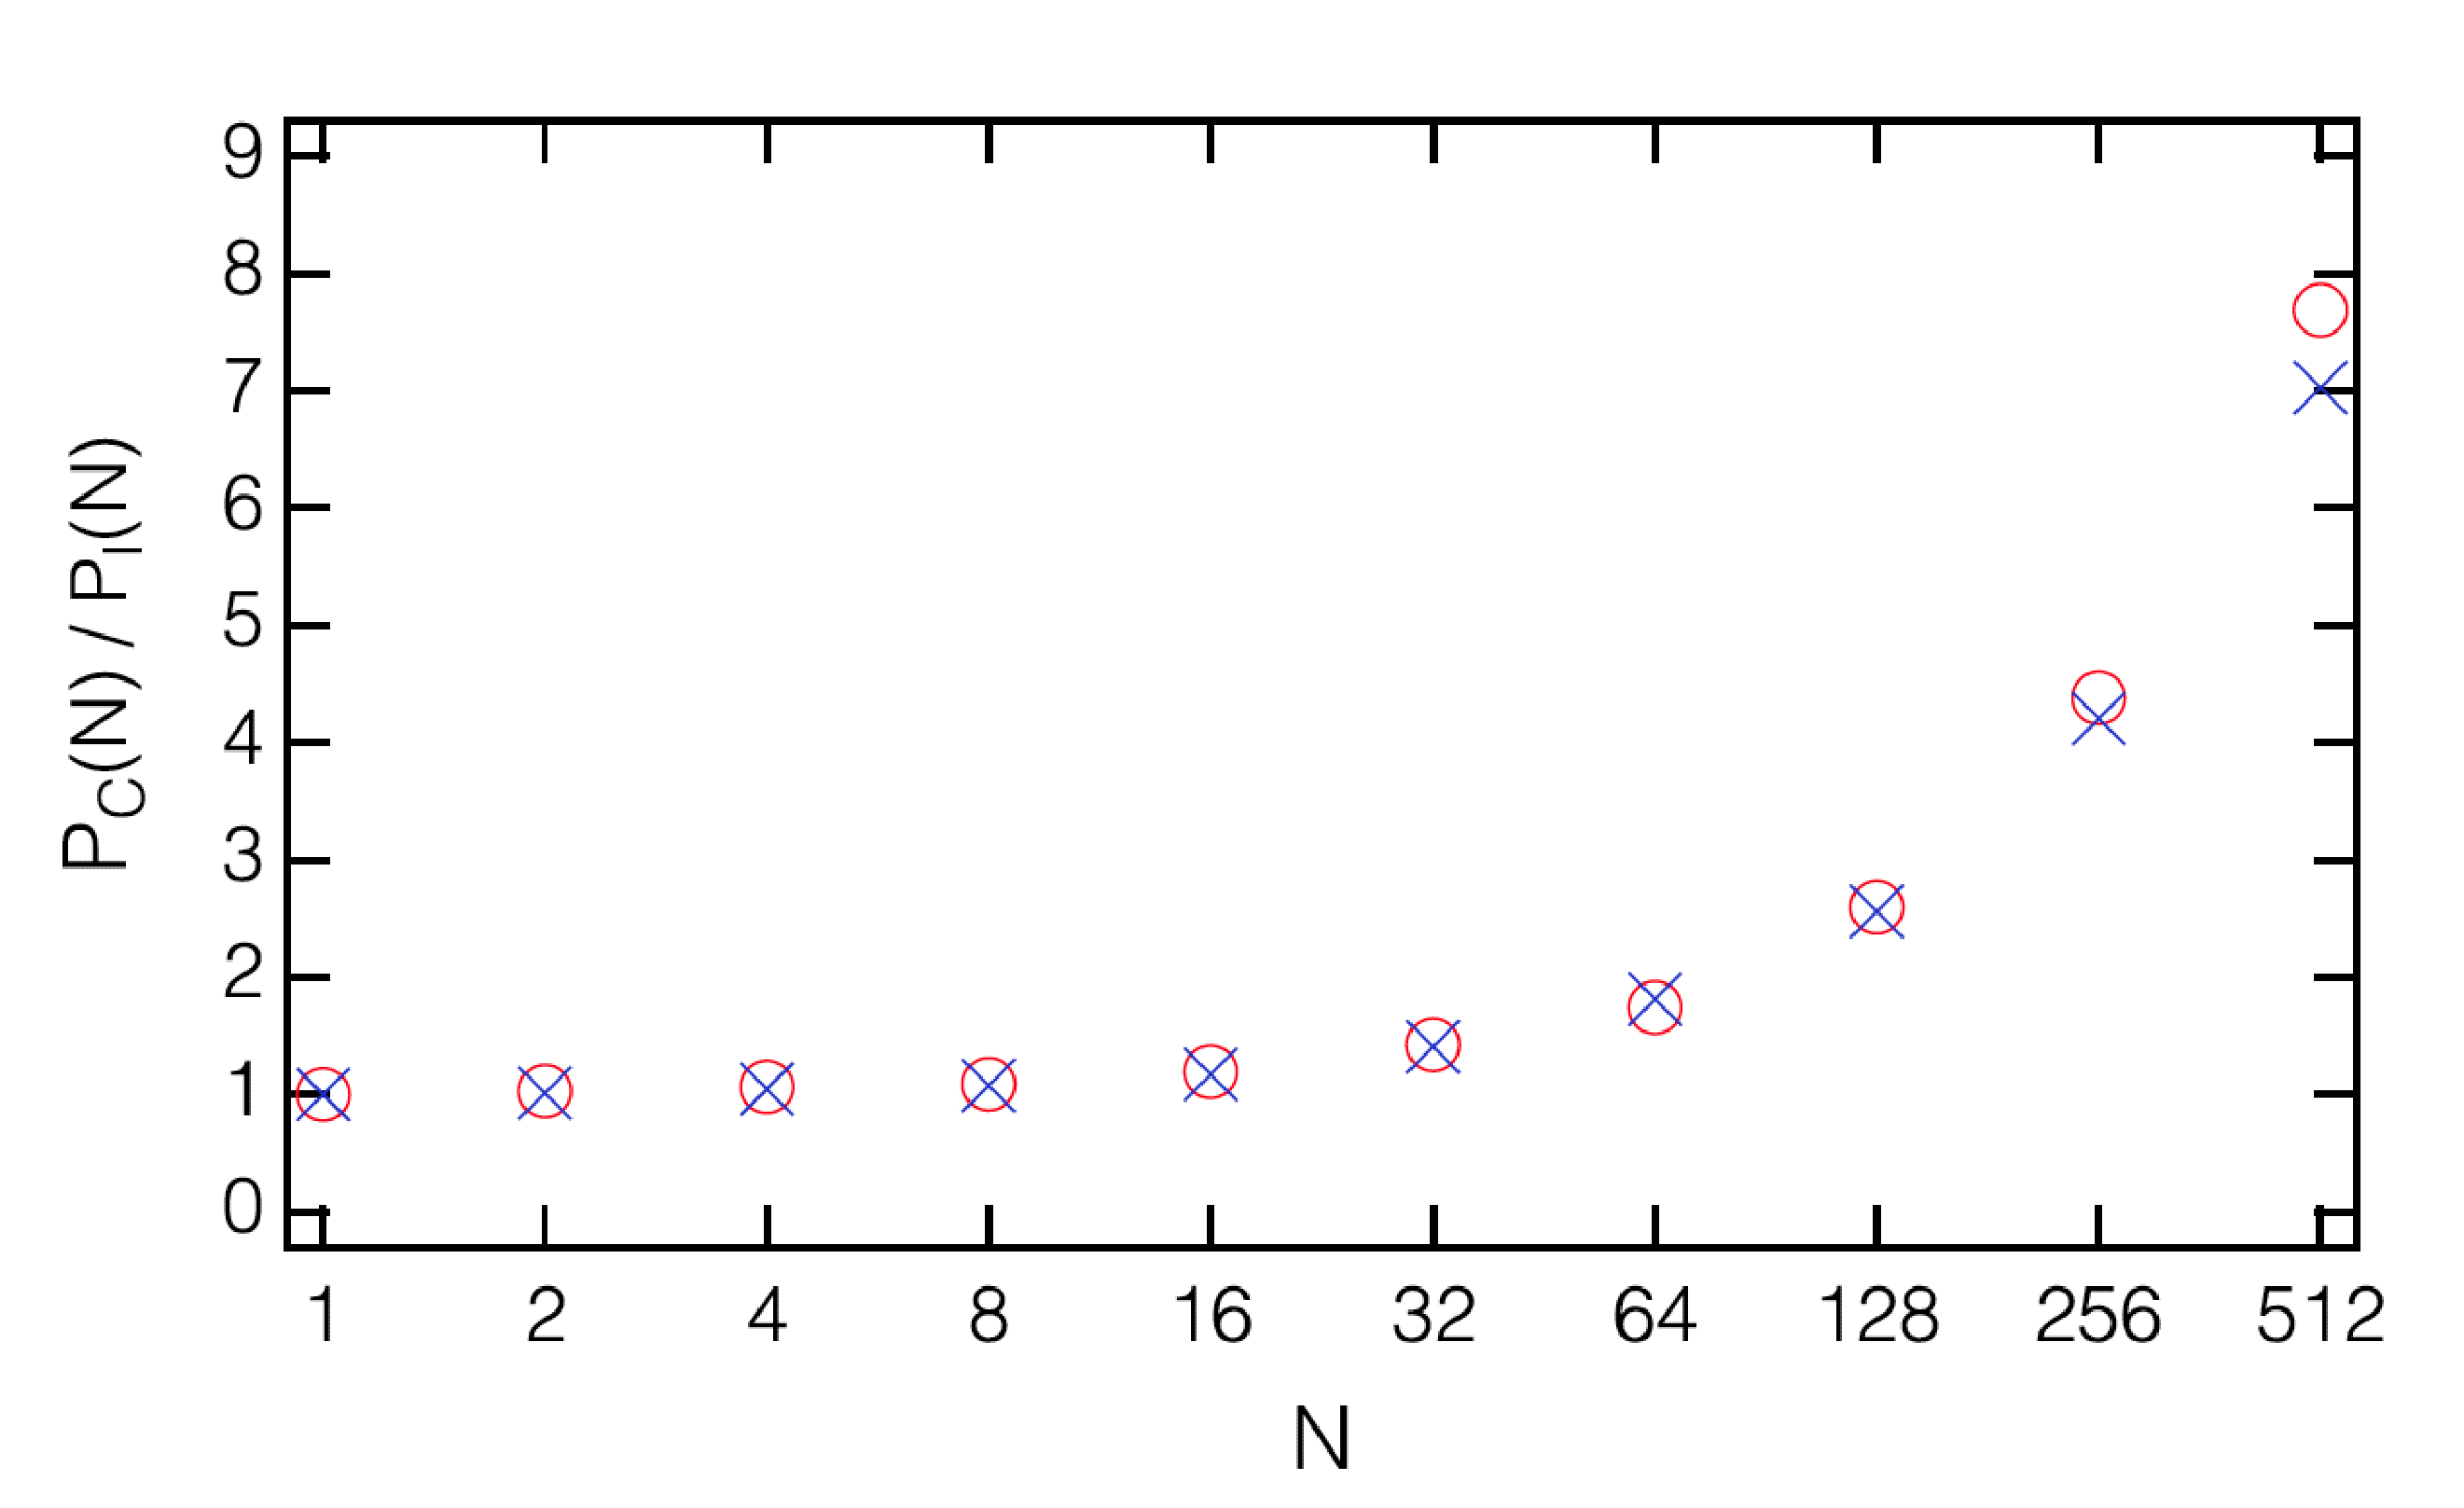
\includegraphics[width=\textwidth]{Pc_Pi.pdf}
\end{center}
%\caption{Log-log plot of the total radiated power vs. the number of atoms from two types of models. $R$=1 and $\delta=600$ in both cases. The solid line is the result of Eq.~\eq{PN}. Ret dots denote the results from simulations.}
\caption{Ratio of the numerically simulated scattered light power to the power from independently radiating atoms plotted for varying atom number $N$ for a Gaussian cloud with the rms radius $R$ satisfying $kR=10$. The detuning is varied in such a way that the estimated optical thickness through the center of the cloud is $10^{-2}$ for all $N$. The circles and crosses are for different signs of the detuning such that the cloud acts as eighteen focusing or a defocusing lens.}
\label{PCANDPN}
\end{figure}



We plot in Fig.~\eq{PCANDPN} the ratio of the numerically simulated collective power to the independent-atom power, $P_C(N)/P_I(N)$, for different number of the atoms $N$. Here the cloud radius give $kR=10$. While we vary the atom number and hence the density, we also vary the detuning in such a way that the estimated optical thickness for a ray going straight through the center of the could is $10^{-2}$, so that absorption of light should not be a major factor. We have both positive (circles) and negative (crosses) detunings that make the gas either a focusing or defocusing lens.

The surprise here is that by $N=128$ when the collectively scattered power already more than doubles the independent-atom power, the central density $n$ of the cloud gives the cooperativity parameter of only $\xi=n\lambdabar^3\sim 0.03$. Our hypothesis is that co-operation sets in much earlier than expected, and we suspect that the same applies elsewhere too.


%The solid line in Fig.~\eq{PCANDPN} reflects the analytical result of a Gaussian cloud of independent radiators as given by Eq.~\eq{PN} and the red scatters represents the results of  radiators with dipole-dipole interactions.  
 
%We notice that the total power with cooperativity exceeds at small atom numbers but the situation reverses at large $N$, where the gas radiates much less then one would expect according to Eq.~\eq{PN}. This is a clear signature of cooperativity (for the only difference in this two models is the presence of light rescattering between atoms. ?)

\section{Shifts of a Resonance Line of Gases in a Circular Disk}

Compared with the total radiated power, the spectroscopic evidence of cooperativity is of more interest to us. To observe this, we replace the Gaussian cloud with a gas sample evenly distributed in a circular-disk-shaped container. This geometry is vastly studied in recent theoretical and experimental research~\cite{PhysRevLett.108.173601}.

As previously mentioned, Lorentz-Lorenz or collective Lamb shifts are expected in a dense atomic sample as cooperative responses to light. 

We have also concluded in Chapter 3 that for a slab configuration, a uniform-density medium restricted to the interval $z\in [0,h]$ and a plane wave with the wave number $k=\omega/c$ propagating in the $z$ direction, in the limit of asymptotically small density $\rho$ of the medium, the absorption line is Lorentzian and is shifted by
\bea
\Delta_L=\Delta_{LL}-\frac{3}{4}\Delta_{LL}\left(1-\frac{\sin 2hk}{2hk}\right);\,\quad\Delta_{LL}=-\frac{\rho\mathcal{D}^2}{3\epsilon_0\hbar}
\label{LL_CLS}
\eea
from the atomic resonance. Here $\Delta_{LL}$, a redshift , is the standard LL shift, and $\Delta_L$ is the CLS as in Ref.~\cite{FRIEDBERG1973101}. In the present formulation the CLS is a combination of the LL shift and the etalon effect because of the reflections of light from the front and back surfaces of the sample. This is the CLS verified in the experiments~\cite{PhysRevLett.108.173601}.

The derivation of the CLS $\Delta_L$ in Ref.~\cite{FRIEDBERG1973101} and many other analyses such as in Ref.~\cite{PhysRevA.81.053821} are all built on a common foundation of mean-field theory. This approximation ignores the correlations between nearby atoms that might arise from dipole-dipole interactions, and as such is uncontrolled. This is why we will solve the light propagation problem using stochastic classical-electrodynamics simulations~\cite{PhysRevA.59.649,PhysRevE.69.026605,PhysRevLett.101.103602,1367-2630-14-5-055001,PhysRevA.86.031602,PhysRevB.86.085116,PhysRevB.86.205128,PhysRevA.88.033844}.

In the simulation, we have $N$ atoms fixed at positions $\br_i,\, i=1,\dots,N$, each with an assumedly isotropic polarizability $\alpha$, we find a closed set of linear equations given by Eq.~\eq{FEQ}. Having solved it numerically, we have the electric field amplitude everywhere as in Eq.~\eq{EF}.

The radius of the circular disk in our numerical experiments is $R=\sqrt{256/\pi}k^{-1}$, so that the area is $A=256k^{-2}$. We vary the thickness of the disk $h$ but keep the density $\rho=N/hA=2k^3$ constant in our examples, so the number of atoms $N$ varies accordingly. A circularly polarized plane wave comes in perpendicular to the pace of the disk. Analogous numerical experiments, although for different purposes, have been described in Refs.~\cite{1367-2630-14-5-055001,PhysRevA.86.031602}.  

We generate a number of random samples, from 64 to millions, of atomic positions evenly distributed inside the disk, compute the absorption as a function of the detuning $\Delta$ for each sample, and average the results. We express the final results in terms of optical thickness $D$ defined as $D=-\ln T$. The advantage is that in a medium that obeys Beer's law the line shape of optical thickness $D$ would be independent of the thickness $h$ of the sample. 

Fig.~\eq{HOMO_D} shows the optical thickness $D$ as a function of detuning $\Delta$ for the sample thicknesses $hk=0.25, 0.5, 1.0$ and $2.0$, with the corresponding atom numbers $N=128, 256, 512,$, and $1024$. For comparison we also give the predicted LL shift of this atom density as the dashed vertical line. The absorption lines are not Lorentzian. While the line broadens with increasing atom number and may be noticeably asymmetric, the maximum moves very little. The shift, if any, is at most a few percent of the LL shift. There is no manifest LL shift, nor a CLS.


\begin{figure}[h!]
\begin{center}
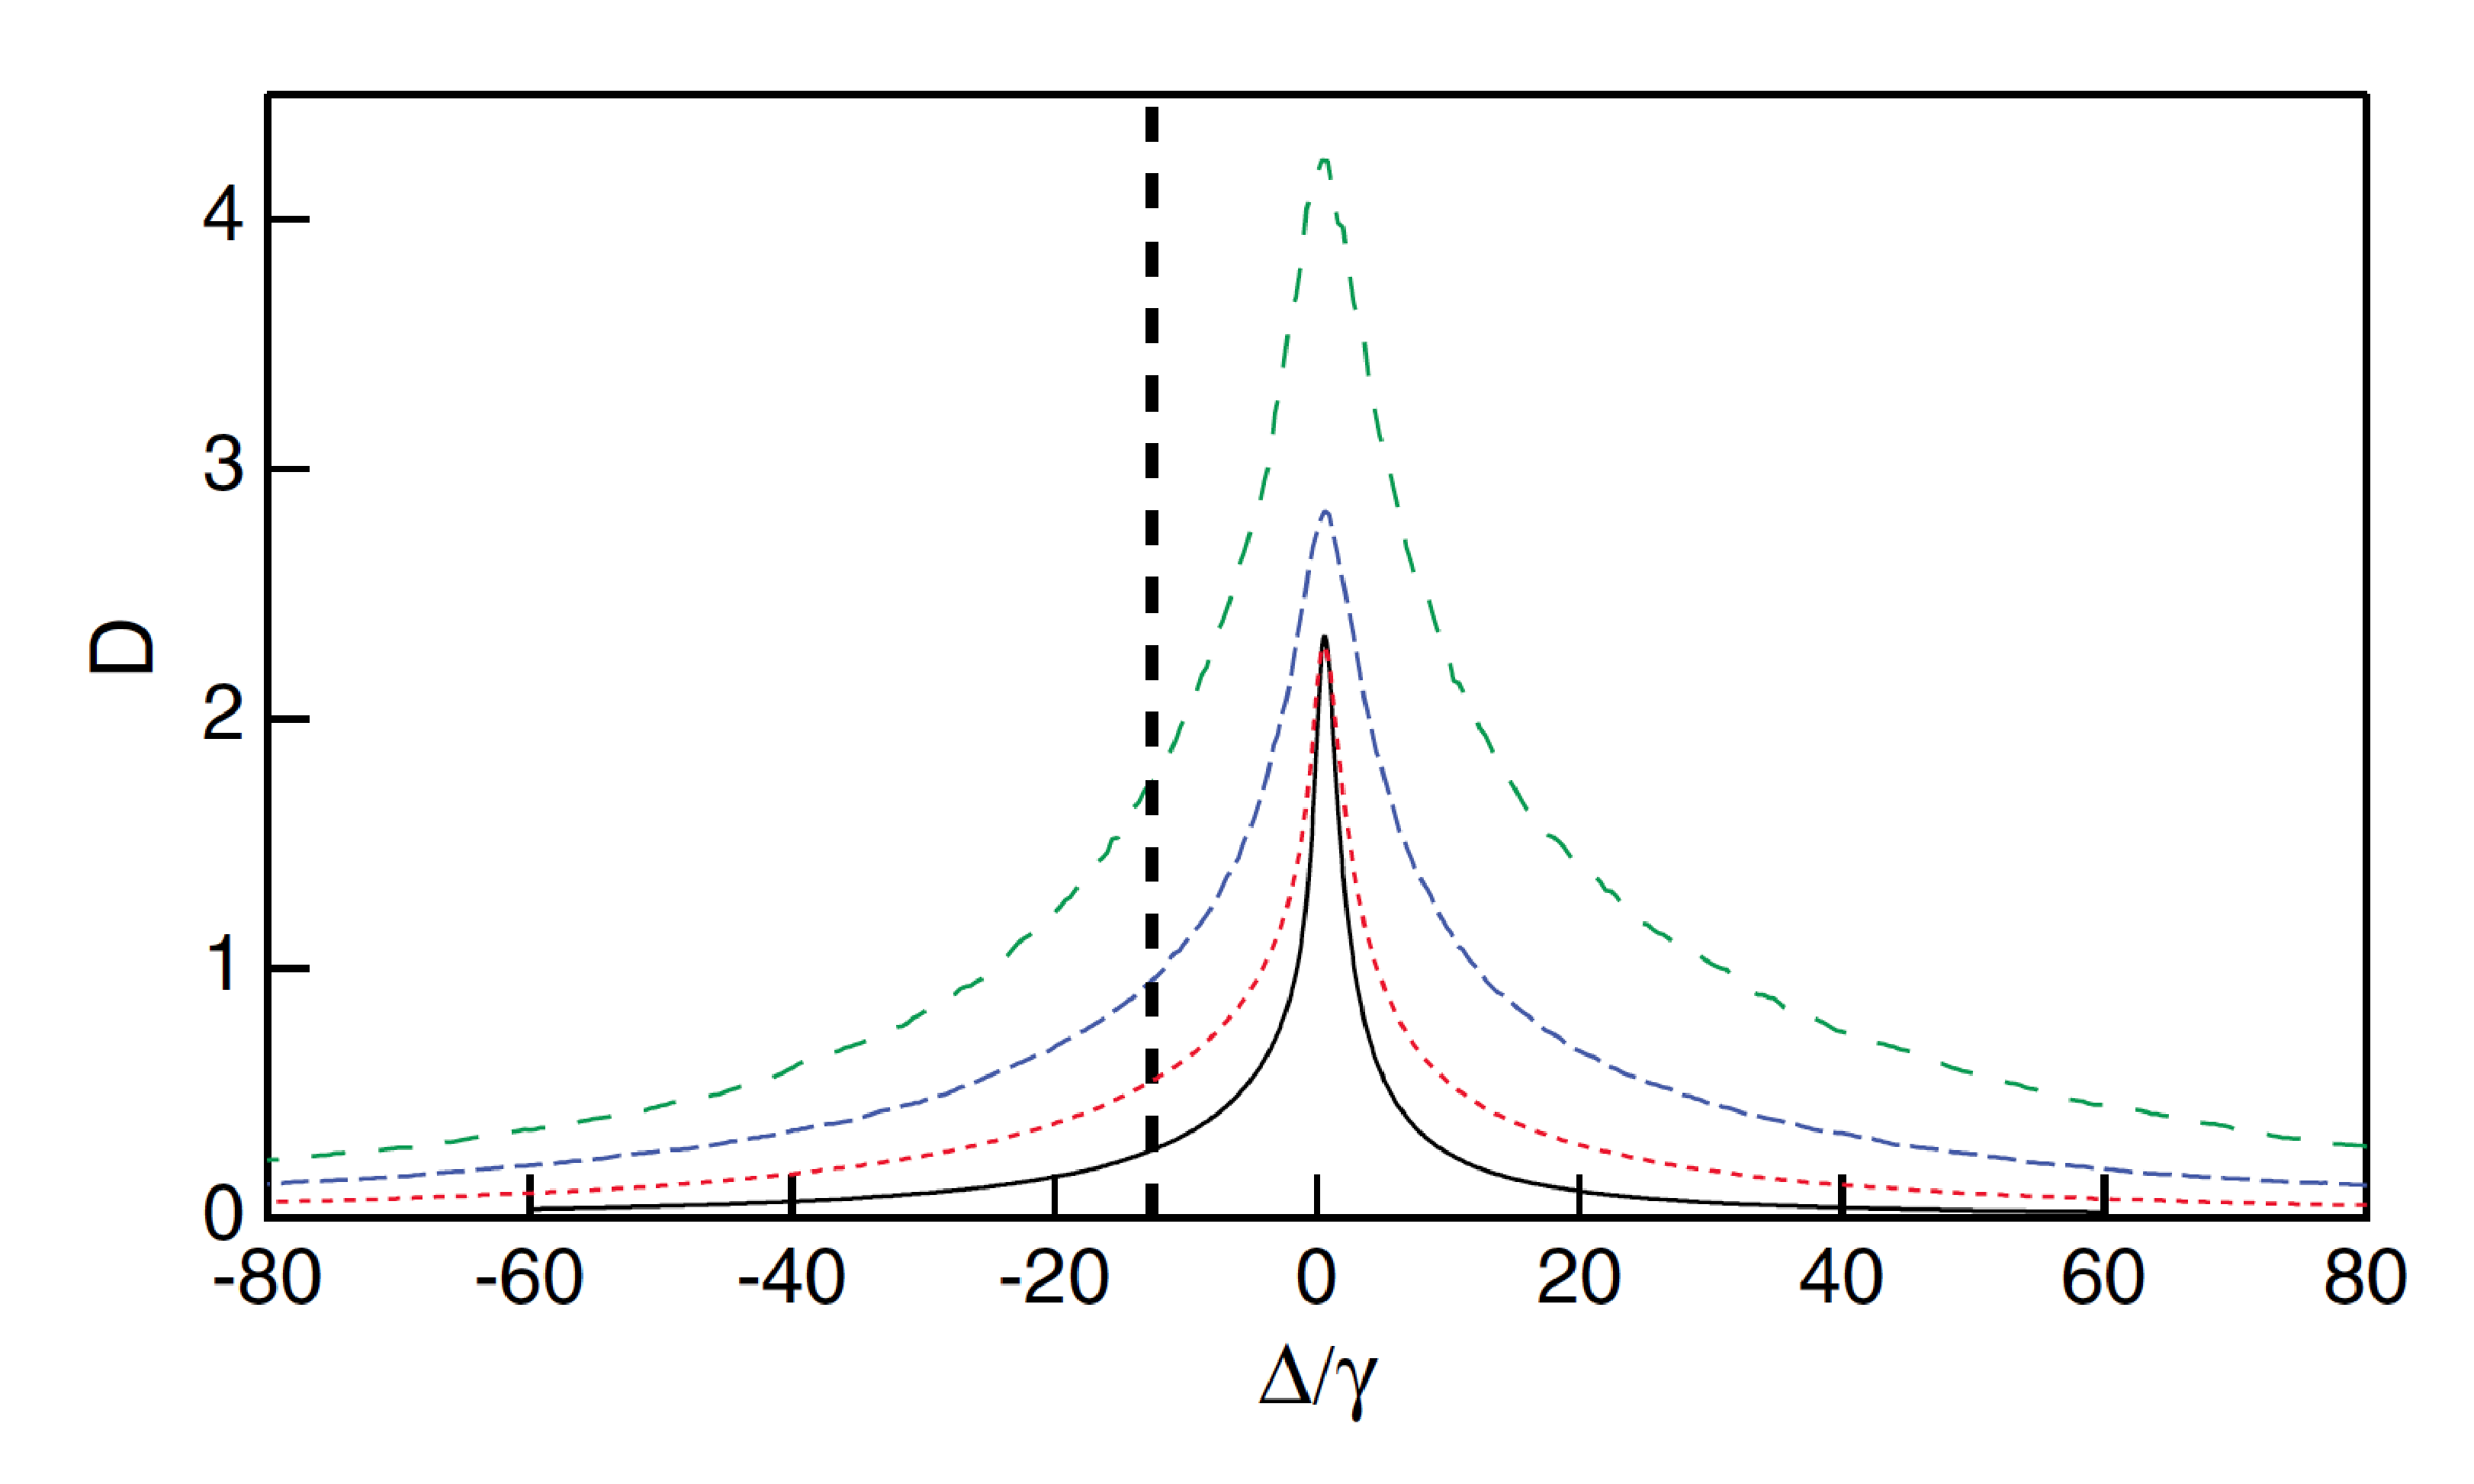
\includegraphics[width=\textwidth]{homo_D.pdf}
\end{center}
\caption{Optical depth $D$ versus detuning $\Delta$ in a homogeneously broadened sample for sample thicknesses $hk=0.25, 0.5, 1.0$, and $2.0$, from bottom to top; the corresponding atom numbers are $N=128, 256, 512,$ and $1024$. The dashed vertical line shows where the center of the line would be if the naive Lorentz-Lorenz shift applied.}
\label{HOMO_D}
\end{figure}

Note that the atoms are fixed in position, this configuration is obviously oversimplified. Therefore, although all correlations between atoms are included in the simulations, we do not observe the density dependent shifts, which are predicted from mean-field theory that ignores the correlations and verified by experiments.

Before introducing new factors into our simulations, such as atomic motions, we simply repeat the numerical experiments with stationary atoms in the circular disk, except that this time we assume that the resonance fequency of each atom is also shifted by a Gaussian random variable with zero mean and the rms value $\omega_D=100\gamma$, which could be interpreted as the effect of Doppler shift depends on the volocity of an atom.

An example spectrum is shown in Fig.~\eq{INHOMO_D}. The line shape has the appearance common in the spectroscopy of inhomogeneously broadened samples. Accordingly, we fit it with the Voigt profile $V(\Delta;\Gamma,\Omega_D)$, convolution of a Lorentzian with the HWHM width $\Gamma$ and a Gaussian with the rms width $\Omega_D$. 

\begin{figure}[h!]
\begin{center}
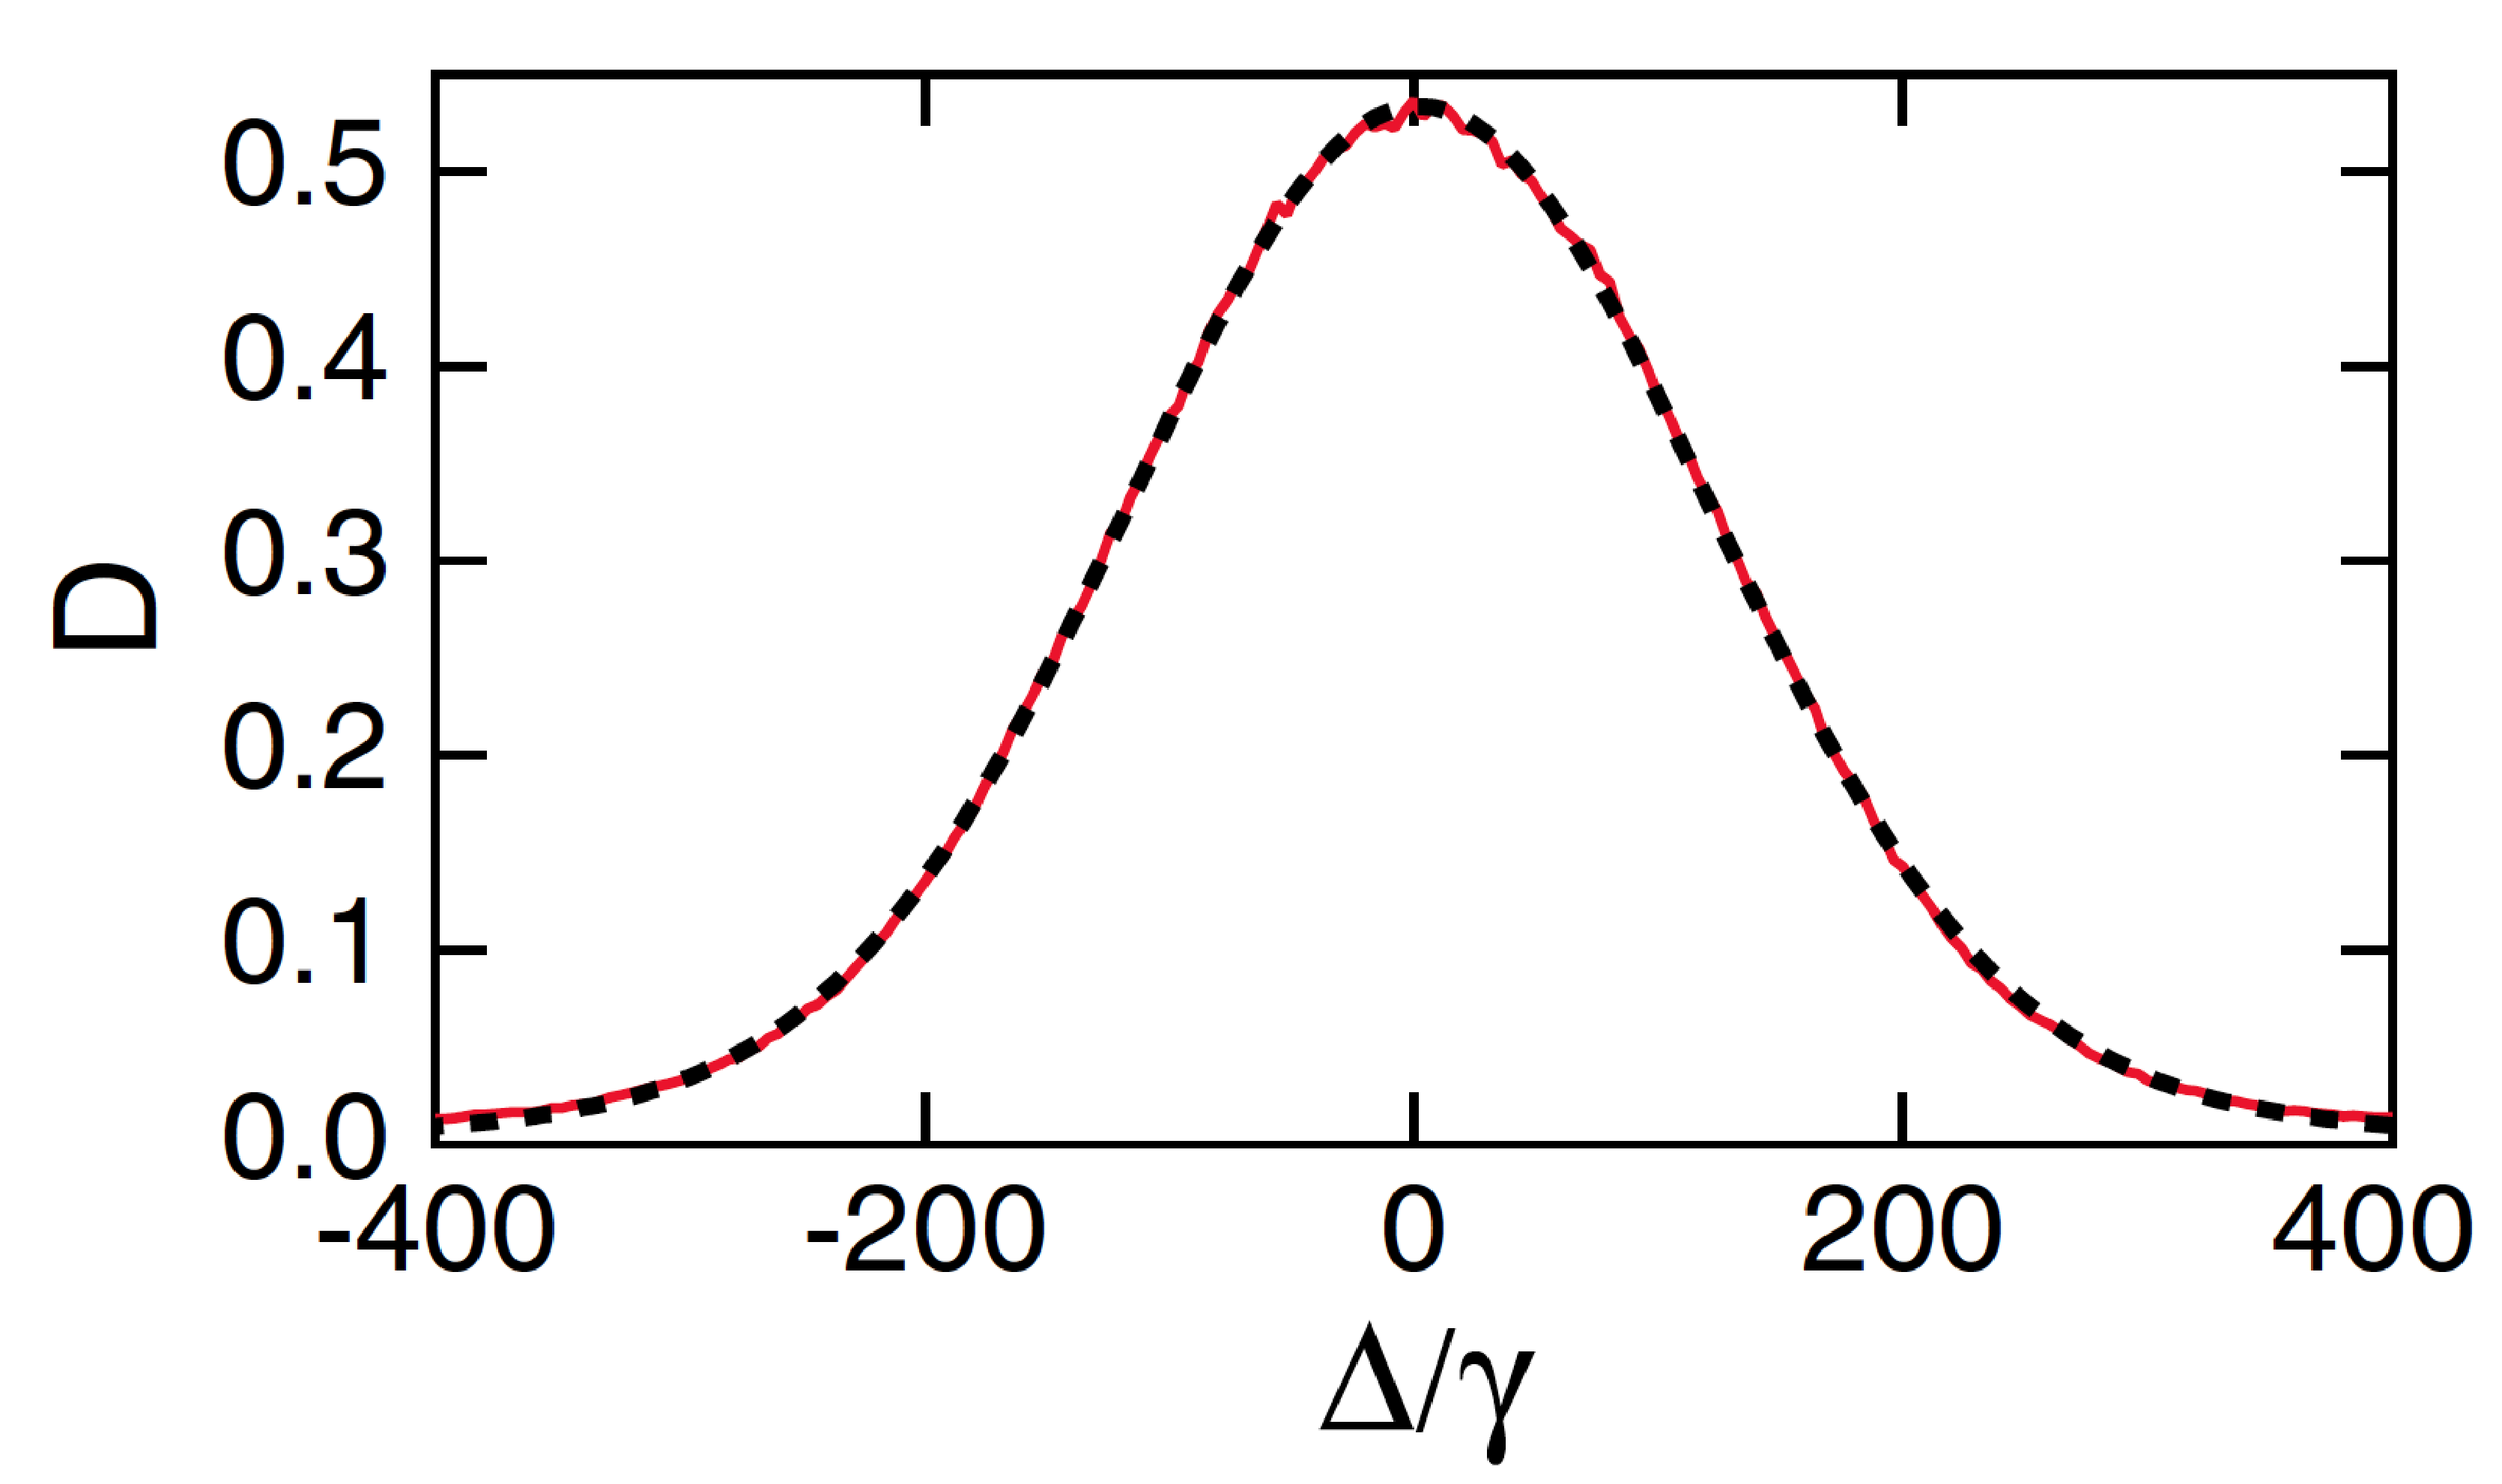
\includegraphics[width=\textwidth]{inhomo_D.pdf}
\end{center}
\caption{Optical depth of the sample $D$ with thickness $hk=1.5$, and, hence, $N=768$ atoms, as a function of the detuning for a sample with the inhomogeneous linewidth $\omega_D=100\gamma$. This numerical experiment (solid red line) is an average of 1024 samples, the fit with a Voige profile (dashed black line) has the parameters $s=2.15\gamma$, $\Gamma=17.74\gamma$, and $\Omega_D=112.83\gamma$.}
\label{INHOMO_D}
\end{figure}

We plot the shift of the resonance $s$ as a function of the thickness of the disk $h$ in Fig.~\eq{STATIC_CLS}, as filled circles. The shift tends to zero at small thicknesses. In this limit the physics becomes two dimensional, for a fixed three-dimensional density the relevant two-dimensional area density tends to zero, and eventually the toms mush radiate completely independently. 

We also plot the CLS, Eq.~\eq{LL_CLS}, as a solid line. Numerical data and theory show similar oscillations, albeit differing approximately by an additive constant. In Fig.~\eq{STATIC_CLS} we also plot as a dashed line the vertically translated version of the theory to fit the numerical data points with $hk\geq 1$. There was an additive term fitted to the experiments~\cite{PhysRevLett.108.173601}, too, before they gave an agreement with Eq.~\eq{LL_CLS}. The agreement of our numerical experiments with the theory is on a similar footing as in the real experiments.


\begin{figure}[h!]
\begin{center}
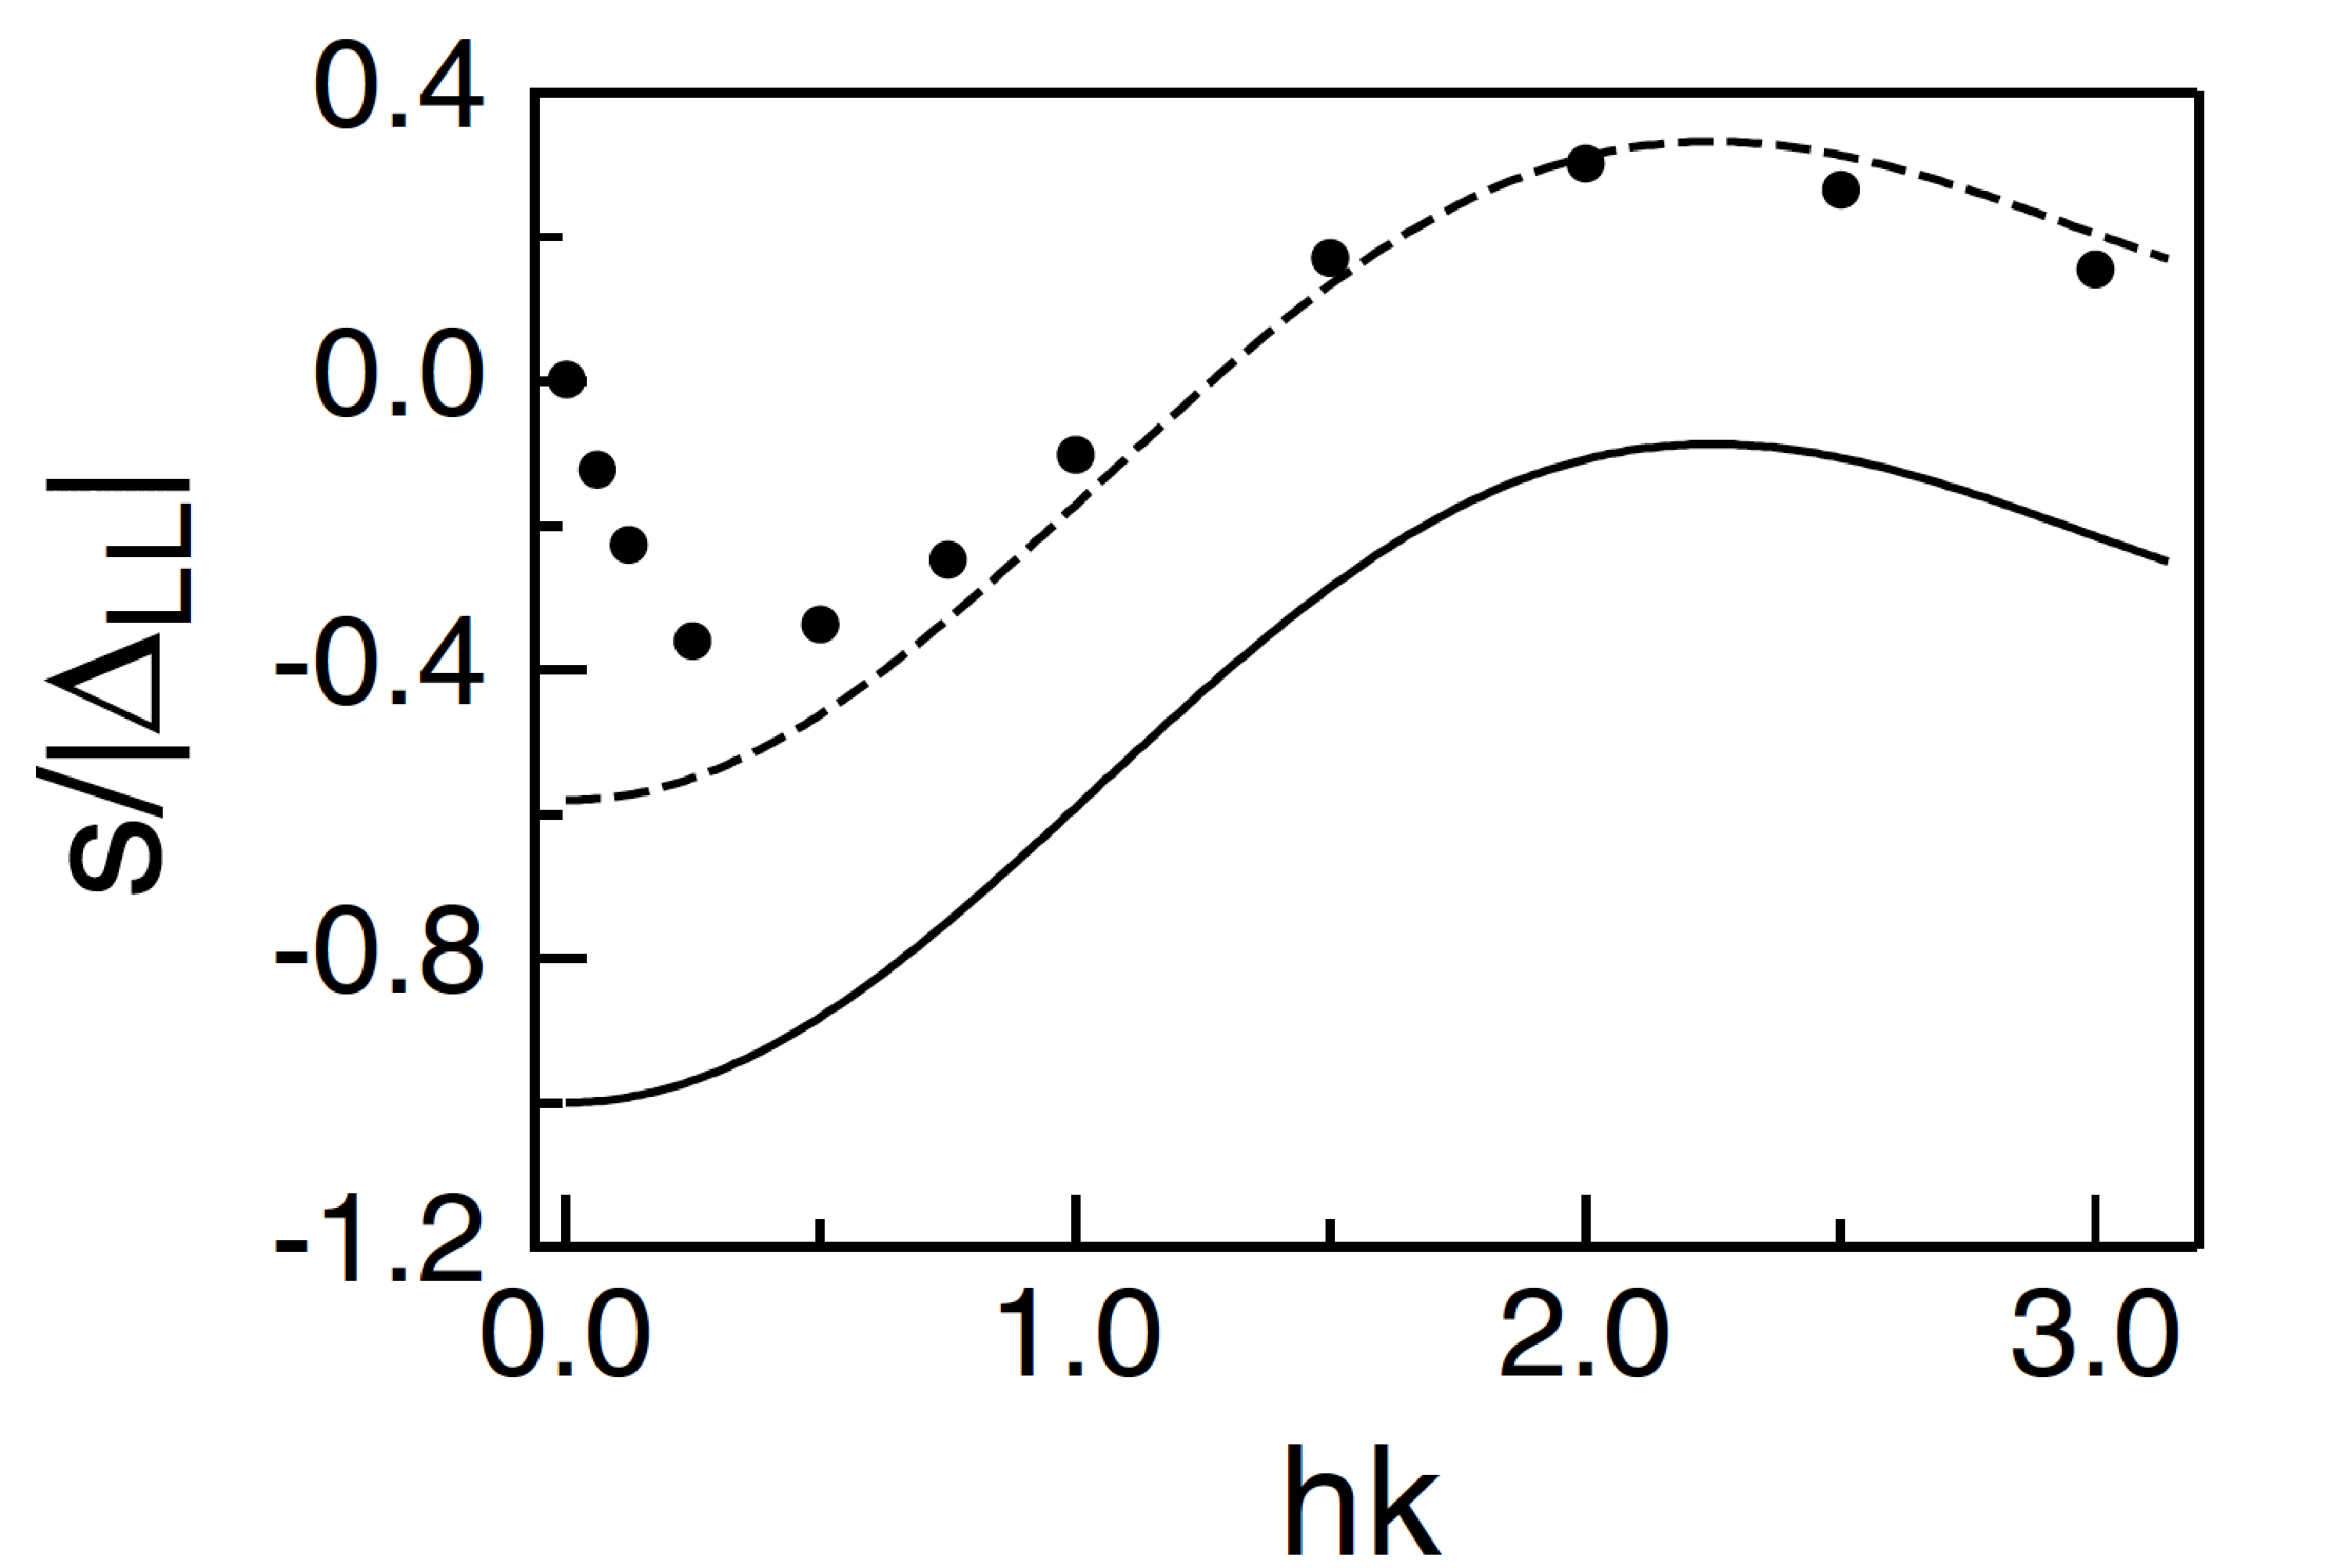
\includegraphics[width=\textwidth]{CLS_static.pdf}
\end{center}
\caption{The sift of the absorption line $s$ lotted as a function of the thickness of the sample $h$ as solid cricles. The statistical error bars are smaller than the size of the circles. Also shown as a solid line is the collective Lamb shift, Eq.~\eq{LL_CLS}, and as a dashed line a vertically translated version of Eq.~\eq{LL_CLS} fitted to the numerical data points with $hk\geq 1$.}
\label{STATIC_CLS}
\end{figure}


The inhomogeneous broadening apparently emphasizes mean-field physics at the expense of correlations between adjacent atoms.

Consider a two-atom sample of atom 1 and 2, with different resonance frequencies, hence, different polarizabilities $\alpha_1$ and $\alpha_2$, we can sketch a formal solution to Eq.~\eq{FEQ}. The field on atom 2 that is generated by the incident field and the light scattered from atom 1 yields
\bea
\bE(\br_2)&=&(1-\alpha_1\alpha_2\G\G)^{-1}[\cbE_0(\br_2)+\alpha_1\G\cbE(\br_1)]\nonumber\\
&=&\cbE_0(\br_2)+\alpha_1\G\cbE_0(\br_1)+\alpha_1\alpha_2\G\G\cbE_0(\br_2)+\dots.
\eea

The second line shows the first three terms of the expansion of $(1-\alpha_1\alpha_2\G\G)$, with $\G\equiv\G(\br_1-\br_2)=\G(\br_2-\br_1)$. The first term is the free field on atom 2; in the second term the free field excites atom 1, which sends its dipolar field back on atom 2; in the third term the free field excites atoms, which sends a dipolar field to excite atom 1, which sends a dipolar field back on atom 2. Further terms in the expansion come out the same way reflecting repeated photon exchanges between the atoms. Such recurrent scattering processes in which a classical wave scatters more than once by the same atom are responsible for the cooperative phenomena and the emergence of subradiant and superradiant resonanes~\cite{PhysRevA.55.513,PhysRevA.86.031602,PhysRevB.86.085116}

Let us now regard atom 2 as the spectator and imagine averaging over the position of atom 1. Upon averaging, the second term becomes the mean-field contribution radiated by an assumedly continuous polarization, and further terms represent repeated photon exchanges between the atoms. 

Next, add the inhomogeneous broadening $\omega_D$. To the order of magnitude, averaging over the resonant frequencies suppresses the polarizability by a factor or $\gamma/\omega_D$. Thus, the first nontrivial term in the expansion corresponding to the mean-field polarization gets suppressed by this small factor, and the higher terms by higher powers of the small quantity $\gamma/\omega_D$. Qualitatively, repeated photon exchanges are deemphasized because in such processes bothe the emitter and the absorber are off resonance.

Analogously, the transition from homogeneously broadened to inhomogeneously broadened phenomenology also takes place in a many-atom sample when the inhomogeneous broadening $\omega_D$ and the effective linewidth $\Gamma$ are comparable. This is, in fact, what we observe in the numerical experiments.

From classical-electordynamics simulations, we have found qualitative features in the optical response of a homogeneously broadened dense atomic sample that are at variance with the time-honored pictures of local-field corrections and collective Lamb shifts. However, an inhomogeneous broadening (random distribution of atomic resonance frequencies) restores the agreement with the traditional theory.

So far, the simulations are based on atoms fixed in position with an artificial inhomogeneous broadening. In the following chapter, real atomic motion will be introduced into the simulations.

